% =====================================================================
%  MacroGraph-AI research paper  --  single-file Overleaf project
%  Compiler : pdfLaTeX (default on Overleaf, TeX Live 2023 or newer)
%  Class    : IEEEtran (conference, two column). To switch to a journal
%             layout change the first line to \documentclass[journal]{IEEEtran}.
%  Figures  : put the folder "research_images" next to this file
%             (upload the folder as it is, with all the PNG images inside it;
%             the path is set by the graphicspath line below).
%  Bibliography is embedded at the bottom, so this one file is enough.
% =====================================================================
\documentclass[conference]{IEEEtran}

% ---------------------------------------------------------------- packages
\usepackage[T1]{fontenc}
\usepackage[utf8]{inputenc}
\usepackage{lmodern}
\usepackage{microtype}
\usepackage[cmex10]{amsmath}
\usepackage{amssymb}
\usepackage{graphicx}
\usepackage{booktabs}
\usepackage{array}
\usepackage{multirow}
\usepackage{xcolor}
\usepackage{algorithm}
\usepackage{algpseudocode}
\usepackage{cite}
\usepackage{xurl}
\usepackage[hidelinks]{hyperref}   % load late
\usepackage[capitalise,noabbrev]{cleveref}

\graphicspath{{research_images/}}

% ---------------------------------------------------------------- macros
\newcommand{\sys}{\textsc{MacroGraph-AI}}
\newcommand{\code}[1]{\texttt{\detokenize{#1}}}
\newcommand{\figref}[1]{\cref{#1}}
\newcommand{\todo}[1]{\textcolor{red}{[#1]}}
\newcommand{\ie}{i.e.,\ }
\newcommand{\eg}{e.g.,\ }
\renewcommand{\algorithmicrequire}{\textbf{Input:}}
\renewcommand{\algorithmicensure}{\textbf{Output:}}
\Crefname{figure}{Fig.}{Figs.}
\crefname{figure}{Fig.}{Figs.}
\Crefname{table}{Table}{Tables}
\crefname{section}{Section}{Sections}
\Crefname{section}{Section}{Sections}
\Crefname{equation}{Eq.}{Eqs.}
\crefname{equation}{Eq.}{Eqs.}
\Crefname{algorithm}{Algorithm}{Algorithms}
\crefname{algorithm}{Algorithm}{Algorithms}
\emergencystretch=1.5em
\hyphenation{Macro-Graph Agent-Cards Fast-MCP Lang-Graph Duck-DB}

\begin{document}

% ================================================================ title
\title{MacroGraph-AI: An Ownership-Constrained, Provenance-Enforced Multi-Agent Architecture with an Evidence-Graded Causal Graph for Verifiable Indian Macroeconomic Analysis}

\author{\IEEEauthorblockN{Nithish Kumar C~S\IEEEauthorrefmark{1},
Hariprasaadh K\IEEEauthorrefmark{1},
Arulprasaad S~J\IEEEauthorrefmark{1},
Tulasi Prasad Sariki\IEEEauthorrefmark{1}}
\IEEEauthorblockA{\IEEEauthorrefmark{1}Department of Computer Science and Engineering (Artificial Intelligence and Machine Learning),\\
Vellore Institute of Technology, Chennai, India\\
Email: \todo{corresponding author email}}}

\maketitle

% ================================================================ abstract
\begin{abstract}
Large language model (LLM) agents can draft fluent macroeconomic commentary, but a single unsupported figure makes a policy brief unusable. We present \sys{}, an open-source multi-agent platform for Indian macroeconomic analysis that enforces provenance in code rather than in prompts. Ten sector agents each own a distinct set of indicators, exchange conclusions only over a typed agent-to-agent (A2A) protocol along seven declared edges, and read data only through their own Model Context Protocol (MCP) tool servers. The protocol server rejects any non-failed response that carries no source, so an unsourced observation cannot reach a report. Cross-sector questions use a causal knowledge graph of 20 indicators and 12 edges on a five-tier evidence taxonomy, and an Edge Evidence Audit labels each edge as expert-seeded or empirically supported by a Granger test. A separate verification library checks typed claims against content-addressed evidence with exact decimal arithmetic and renders only verified text. We report what the implementation does and does not do. On the bundled data none of the 12 edges is testable, which exposes a data-depth gap that graph-augmented systems rarely surface. The scenario engine is an attenuation heuristic and not an identified model, and the verification library is not yet integrated into the orchestrator. We give formal definitions of each mechanism and a pre-specified evaluation (five systems, three ablations, 240 questions) that must be completed before any accuracy claim is made.
\end{abstract}

\begin{IEEEkeywords}
multi-agent systems, large language models, agent-to-agent protocol, Model Context Protocol, causal knowledge graph, provenance, claim verification, macroeconomic analysis, India
\end{IEEEkeywords}

% ================================================================ I. intro
\section{Introduction}
\label{sec:intro}

A central bank analyst asked about the effect of an oil shock on Indian inflation needs numbers from at least four institutions: consumer prices from the Ministry of Statistics and Programme Implementation (MoSPI), the policy rate from the Reserve Bank of India (RBI), the trade balance from the Ministry of Commerce, and exchange-rate data from the market. These releases differ in frequency, base year and publication format, and they are rarely served through a single interface. The analyst then has to join them, remember which series moves which, and cite everything. An LLM can compress this work into a paragraph in seconds, but a paragraph is only useful if each number in it can be traced to a published table and a period. LLMs are known to produce fluent statements that are not supported by their inputs \cite{ji2023hallucination}, and attribution to a source is a distinct property that has to be measured rather than assumed \cite{rashkin2023ais,gao2023alce}.

Recent work has applied LLM agents to economics and finance. EconAgent simulates macroeconomic activity with LLM-driven households and firms \cite{li2024econagent}; TradingAgents organises LLM roles after a trading firm \cite{xiao2024tradingagents}; Hao and Xie map different LLMs to heterogeneous economic agents for policy analysis \cite{hao2025mlab}; and Kato proposes an agentic ``AI economist'' that grounds report generation in knowledge graphs and explicit model computations \cite{kato2026aieconomist}. These systems establish that agent decomposition is useful. In the first pages of the six closest systems (\cref{tab:related}), the stated designs concern agent roles, graph structure or model grounding; none describes a protocol-level rule that rejects unsourced agent output, and none labels its graph edges by empirical support (the full papers may contain such features that we did not see). That leaves open a narrower engineering question that matters for institutional use: \emph{what stops an agent from stating a figure that no data source supports, and what stops two agents from reporting different values for the same indicator?}

This paper presents \sys{}, which answers that question with structure. The contribution is not a larger model or a new prompt; it is a set of constraints that are enforced by code and can be audited. \Cref{fig:architecture} gives the overall picture.

\begin{figure}[t]
\centering
% IMAGE 01 -- System architecture (layered view)
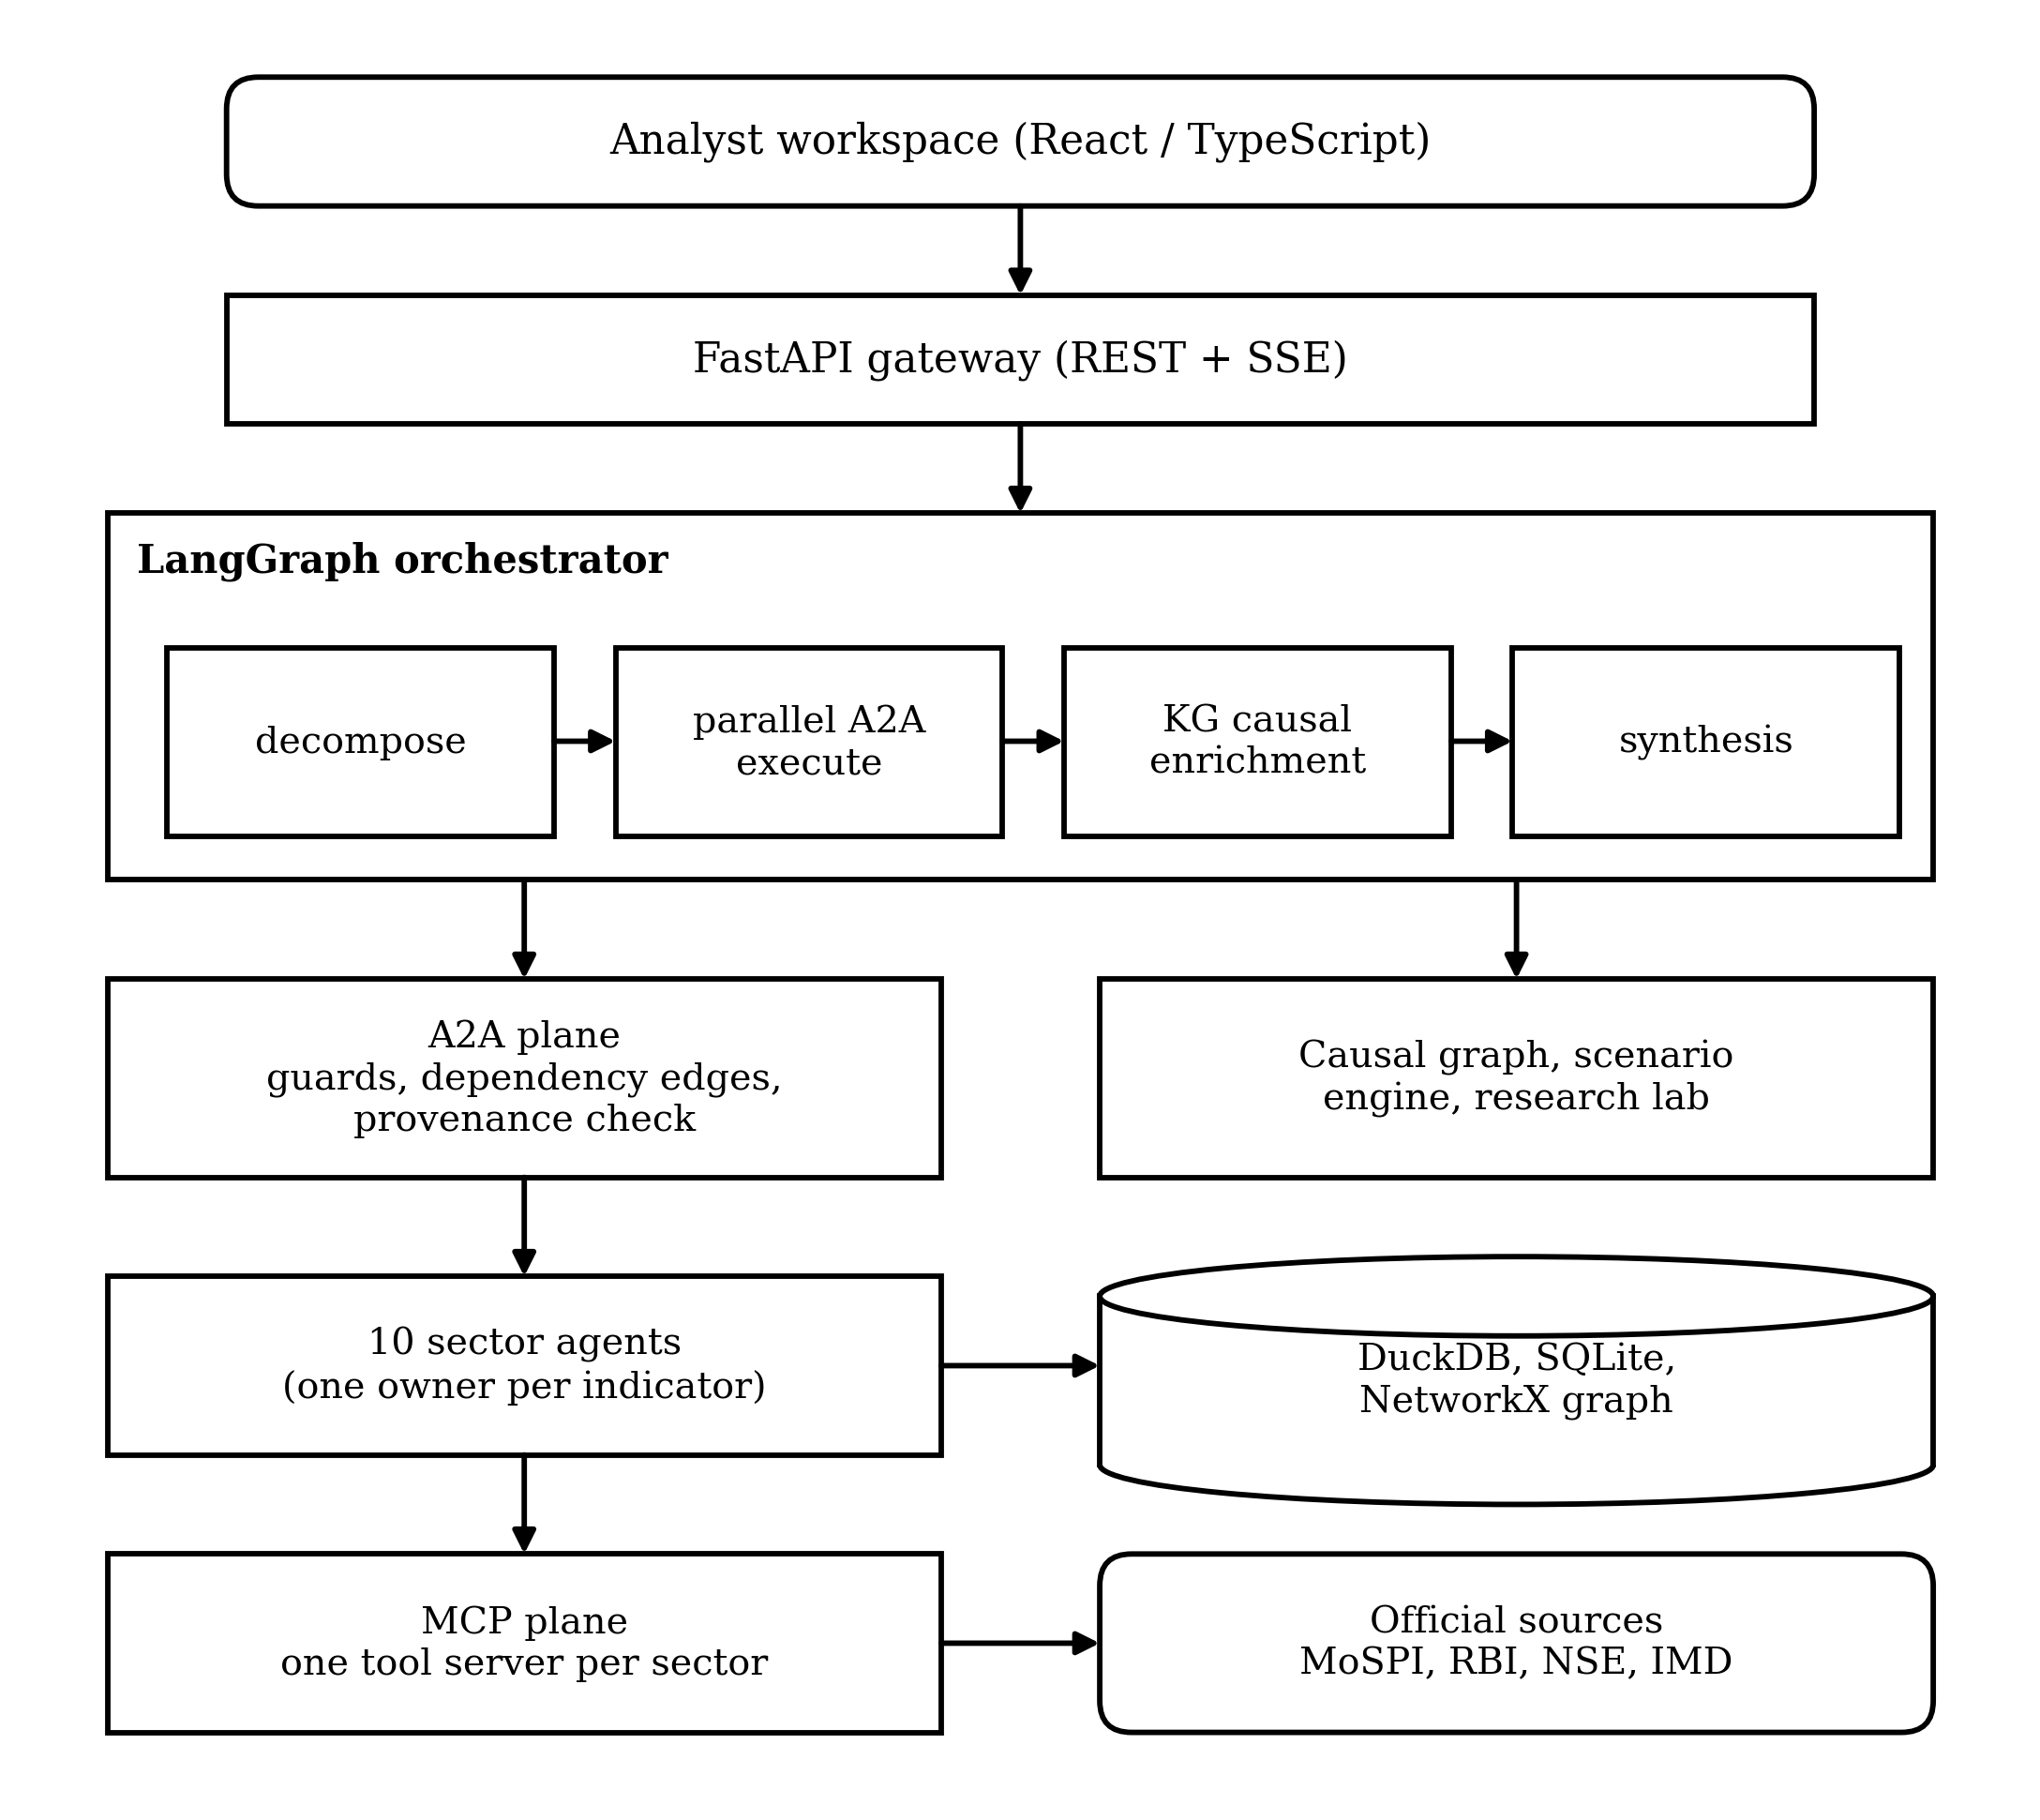
\includegraphics[width=\columnwidth]{01_system_architecture.png}
\caption{Layered architecture of \sys{}. The A2A plane carries agent-to-agent reasoning; the MCP plane carries agent-to-data requests. The causal knowledge graph and the research lab sit beside the orchestrator and are read-only consumers of the agents' output.}
\label{fig:architecture}
\end{figure}

\subsection{Contributions}
We make the following contributions. Each is a property of the released code, and \cref{sec:eval} states exactly how much of it has been tested.

\begin{enumerate}
\item \textbf{Ownership-constrained agent architecture (\cref{sec:design}).} A single-owner-per-indicator rule, a closed set of declared sector-to-sector A2A edges enforced by the protocol server, and per-sector MCP tool servers together separate agent-to-agent reasoning from agent-to-data access. The protocol rejects sourceless responses (``no source, no answer'').
\item \textbf{Evidence-graded causal knowledge graph (\cref{sec:kg}).} A 20-indicator, 12-edge graph with stable relation identifiers and a five-tier evidence taxonomy, and an Edge Evidence Audit that distinguishes \code{SEEDED} edges from \code{EMPIRICAL} ones and reports untestable edges as untestable instead of guessing.
\item \textbf{A transparent scenario baseline (\cref{sec:scenario}).} A closed-form graph-attenuation model whose formula, constants and limitations are written into every answer through a model card. We present it as a named weak baseline, not as an identified structural model.
\item \textbf{Honesty-labelled research lab (\cref{sec:lab}).} Trajectory, twin attribution, graph-conditioned anomaly classification, a simulated six-seat monetary-policy committee and a consensus rollup, all tagged \code{LIVE}, \code{CACHED}, \code{SIM}, \code{SEEDED} or \code{heuristic}.
\item \textbf{Claim-level verification library (\cref{sec:verify}).} Typed claims, content-addressed evidence, exact decimal comparison and deterministic rendering, with an append-only audit trail.
\item \textbf{A candid self-audit and an evaluation protocol (\cref{sec:eval,sec:discussion}).} Measured engineering facts, the audit result on the bundled data, a list of known defects, and a pre-specified evaluation design.
\end{enumerate}

The paper is organised as follows. \Cref{sec:related} reviews related work. \Cref{sec:design} presents the architecture and protocols. \Cref{sec:kg,sec:scenario} describe the knowledge graph and scenario engine. \Cref{sec:lab,sec:verify} cover the research lab and the verification library. \Cref{sec:eval} reports what has been measured and specifies the planned evaluation. \Cref{sec:discussion} discusses limitations and \cref{sec:conclusion} concludes.

% ================================================================ II. related
\section{Related Work}
\label{sec:related}

\paragraph{LLM agents and multi-agent frameworks.}
ReAct interleaves reasoning with tool calls \cite{yao2023react}; generative agents add memory and planning for simulated social behaviour \cite{park2023generative}; AutoGen and MetaGPT structure collaboration among multiple role-specialised agents \cite{wu2023autogen,hong2024metagpt}. Surveys catalogue the design space \cite{wang2024agentsurvey,guo2024masurvey}. Our orchestrator is conventional in this respect. Its distinguishing feature is a protocol server that makes some multi-agent behaviours impossible by construction (cross-sector calls that are not declared, loops, and responses without sources).

\paragraph{Agent communication standards.}
The Model Context Protocol standardises how a model-facing client reaches tools and data \cite{mcp2024}, and the Agent2Agent protocol targets interoperability between independent agents \cite{a2a2025}. We use the two for different purposes and never conflate them: A2A carries delegation and structured conclusions between agents, MCP carries data requests from an agent to a source. Our A2A layer is a project-native implementation shaped after the public specification; we have not tested interoperability with external A2A clients and do not claim it.

\paragraph{Agents for economics and finance.}
EconAgent equips LLM agents with perception, memory and decision modules to reproduce macroeconomic phenomena \cite{li2024econagent}. The AI Economist uses reinforcement learning to design tax policy in a simulated economy \cite{zheng2022aieconomist}. Hao and Xie vary the underlying LLM, not only the prompt, to obtain heterogeneous agents \cite{hao2025mlab}, and Lin et al.\ build LLM agents that simulate macroeconomic expectations in survey experiments and compare them with human data \cite{lin2026expectations}. TradingAgents reports gains over baselines in simulated trading \cite{xiao2024tradingagents}. BloombergGPT is a domain-specific language model for finance \cite{wu2023bloomberggpt}. These works simulate agents that \emph{behave} economically. \sys{} is different in purpose: its agents do not simulate households or traders but retrieve and reconcile published statistics for a human analyst.

\paragraph{Retrieval, knowledge graphs and grounding.}
Retrieval-augmented generation grounds answers in retrieved text \cite{lewis2020rag}. Graph-based variants use structure to organise retrieval, for example community summaries for global questions \cite{edge2024graphrag} or knowledge-graph-guided chunk expansion \cite{zhu2025kg2rag}; Pan et al.\ survey the roadmap for unifying LLMs and knowledge graphs \cite{pan2024llmkg}. Dadopoulos et al.\ show that embedding LLM-generated metadata with chunks improves retrieval on financial filings \cite{dadopoulos2025metadata}. In macroeconomics, Yang et al.\ build a knowledge graph from text and use it as a prior for variable selection in forecasting \cite{yang2020kgmacro}. Closest in spirit, Kato's AI economist combines knowledge graphs, retrieval and explicit model computation so that quantitative claims come from models and not from the language model alone \cite{kato2026aieconomist}. Our graph differs in two ways: it is small and curated, and every edge carries an explicit evidence class that is propagated into answers, with untestable edges declared as such. We do \emph{not} implement document retrieval; documentary evidence is reported as unavailable in every report.

\paragraph{Attribution, fact checking and provenance.}
Attribution measures whether a statement can be traced to a source \cite{rashkin2023ais}, citation generation benchmarks test whether models cite correctly \cite{gao2023alce}, and fact-verification datasets such as FEVER cast the task as claim verification against evidence \cite{thorne2018fever}. W3C PROV defines a general provenance model \cite{belhajjame2013prov}. Our verification library borrows the discipline of typed claims and deterministic checks, but applies it to numeric statistics where an exact check exists, and refuses to certify causation from quoted text.

\paragraph{Econometric background.}
The attenuation model in \cref{sec:scenario} is not an econometric estimator. The standard alternatives are vector autoregressions \cite{sims1980macro} and local projections \cite{jorda2005lp}; predictive causality is commonly tested with Granger's criterion \cite{granger1969}, which requires stationary series \cite{dickey1979,kpss1992} and corrections for multiple tests \cite{bh1995}. Pearl's framework makes explicit what a causal claim requires beyond predictive precedence \cite{pearl2009}. \Cref{sec:discussion} uses these references to state what is missing.

\begin{table*}[t]
\centering
\caption{Positioning against the closest published systems, based on the stated aims and evaluations in the cited abstracts. ``Quantitative evaluation'' means an evaluation reported by the authors of that work; our entry is ``not yet'' because the planned evaluation in \cref{sec:eval} has not been run.}
\label{tab:related}
\small
\begin{tabular}{@{}p{3.7cm}p{3.9cm}p{1.8cm}p{1.9cm}p{4.0cm}@{}}
\toprule
\textbf{System} & \textbf{Primary task} & \textbf{Multi-agent} & \textbf{Knowledge graph} & \textbf{Quantitative evaluation reported} \\
\midrule
EconAgent \cite{li2024econagent} & Simulating macroeconomic activity & Yes & No & Yes (reproduces macro phenomena) \\
TradingAgents \cite{xiao2024tradingagents} & Stock trading decisions & Yes & No & Yes (returns, Sharpe, drawdown) \\
MLAB \cite{hao2025mlab} & Policy impact on heterogeneous agents & Yes & No & Case study (interest-income tax) \\
KG2RAG \cite{zhu2025kg2rag} & Question answering over documents & No & Yes & Yes (HotpotQA variants) \\
Yang et al.\ \cite{yang2020kgmacro} & Variable selection for forecasting & No & Yes & Yes (forecast accuracy) \\
AI Economist Agent \cite{kato2026aieconomist} & Model-grounded economic reports & Yes & Yes & Two applications \\
\midrule
\textbf{\sys{} (this work)} & Cited cross-sector Indian macro analysis with enforced provenance & Yes & Yes & \textbf{Not yet}; engineering tests only \\
\bottomrule
\end{tabular}
\end{table*}

% ================================================================ III. design
\section{System Design}
\label{sec:design}

\subsection{Design principles}
Three principles shape the system and trace back to the failure modes above.

\begin{enumerate}
\item \textbf{One owner per indicator.} Exactly one sector agent is responsible for each primary indicator (\cref{tab:ownership}). Other agents obtain it from the owner, never from the source. This removes the possibility that two agents fetch the same series through different routes and report different values.
\item \textbf{Separate the reasoning plane from the data plane.} Agents talk to one another over A2A and to data over MCP. A sector package never imports another sector package.
\item \textbf{No source, no answer.} Every observation carries its source, table, value, unit, observation period, a \code{data_status} and a SHA-256 \code{provenance_hash}. Missing data produces a structured unavailable status, never an estimate.
\end{enumerate}

\begin{table}[t]
\centering
\caption{Indicator ownership and declared A2A consumers.}
\label{tab:ownership}
\footnotesize
\begin{tabular}{@{}p{2.55cm}p{2.9cm}p{2.0cm}@{}}
\toprule
\textbf{Owner} & \textbf{Primary indicators} & \textbf{A2A consumers} \\
\midrule
\code{prices_sector} & CPI, WPI, sub-indices & Finance, Fiscal, External \\
\code{monetary_sector} & Repo, SDF, MSF, M3 & Finance, Fiscal, External \\
\code{finance_sector} & Credit growth, GNPA, WALR & Fiscal \\
\code{fiscal_sector} & Deficit, GST, capex & -- \\
\code{capital_market_sector} & NIFTY, VIX, FII/DII & -- \\
\code{external_sector} & Trade, reserves, USD/INR & -- \\
\code{real_sector} & GDP, GVA, IIP, GFCF & -- \\
\code{labour_sector} & PLFS, EPFO & -- \\
\code{services_sector} & Services GVA, PMI & -- \\
\code{agriculture_sector} & Crops, MSP, monsoon & -- \\
\bottomrule
\end{tabular}
\end{table}

\subsection{Declared dependencies}
Of the 90 possible ordered sector pairs, the protocol permits seven (\cref{fig:deps}): Finance consumes the repo rate and headline CPI, Fiscal consumes the repo rate, CPI and bank credit growth, and External consumes the repo rate and CPI. Any other sector-to-sector request is returned as \code{DEPENDENCY_NOT_ALLOWED}. The orchestrator is the only component allowed to call every agent. We deliberately left several economically plausible links unwired (\eg Prices--Agriculture) because the provider has no peer-facing task yet; a declared edge is a commitment that the provider can answer.

\begin{figure}[t]
\centering
% IMAGE 02 -- Ownership and declared A2A dependencies
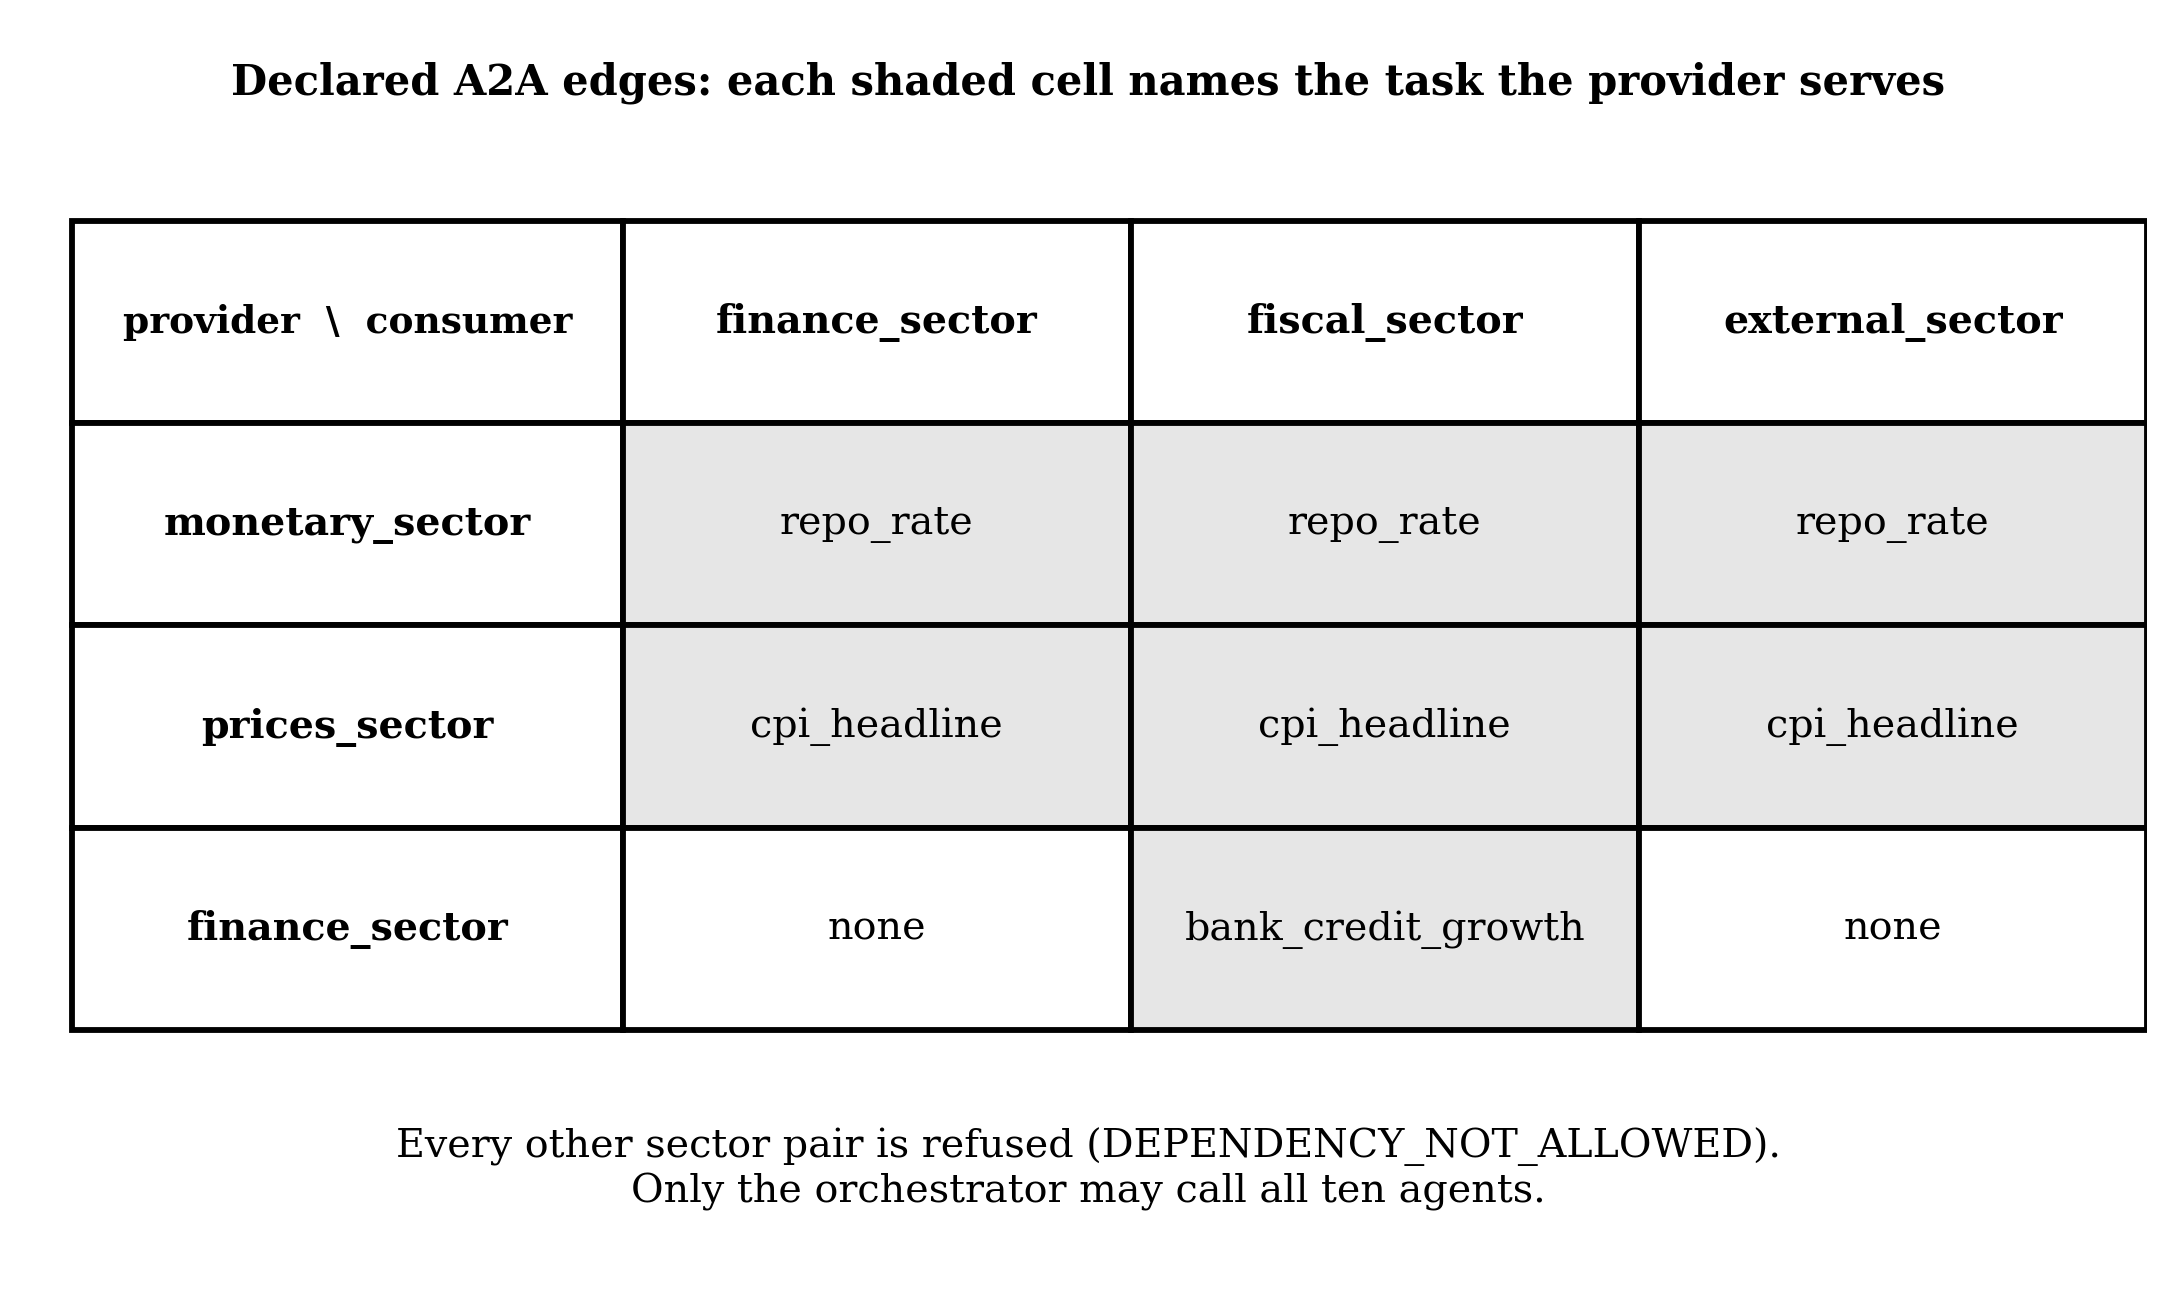
\includegraphics[width=\columnwidth]{02_ownership_dependencies.png}
\caption{Declared sector-to-sector A2A edges. Rows are providers, columns are consumers, and each shaded cell names the task the provider serves. Finance consumes \code{repo_rate} and \code{cpi_headline}; Fiscal consumes \code{repo_rate}, \code{cpi_headline} and \code{bank_credit_growth}; External consumes \code{repo_rate} and \code{cpi_headline}. All other pairs are refused.}
\label{fig:deps}
\end{figure}

\subsection{The A2A protocol}
An A2A request is a frozen, strictly typed record containing a request identifier, sender, receiver, task, parameters, a conversation identifier, the parent request, a delegation depth and the call chain. \Cref{fig:a2apipeline} shows how the server processes it. The delegation guard enforces a maximum depth (default 5), a maximum number of requests per conversation (25), detection of a receiver that already appears on the call chain, and detection of a duplicate request that differs only in identifier. The server then checks that the sector edge is declared and that the task appears in the receiver's Agent Card, runs the handler under a timeout, and validates the response: schema, correlation identifier and, for any non-failed response, a non-empty list of sources.

Failures never propagate as exceptions across agents. They are returned as a typed response with a machine-readable code (\eg \code{AGENT_TIMEOUT}, \code{CIRCULAR_DELEGATION}, \code{INVALID_RESPONSE}). Only timeouts and transport failures are retried, with exponential back-off and the same request identifier. A per-conversation trace store reconstructs the delegation tree; it currently lives in memory and is bounded.

\begin{figure*}[t]
\centering
% IMAGE 03 -- A2A request handling pipeline
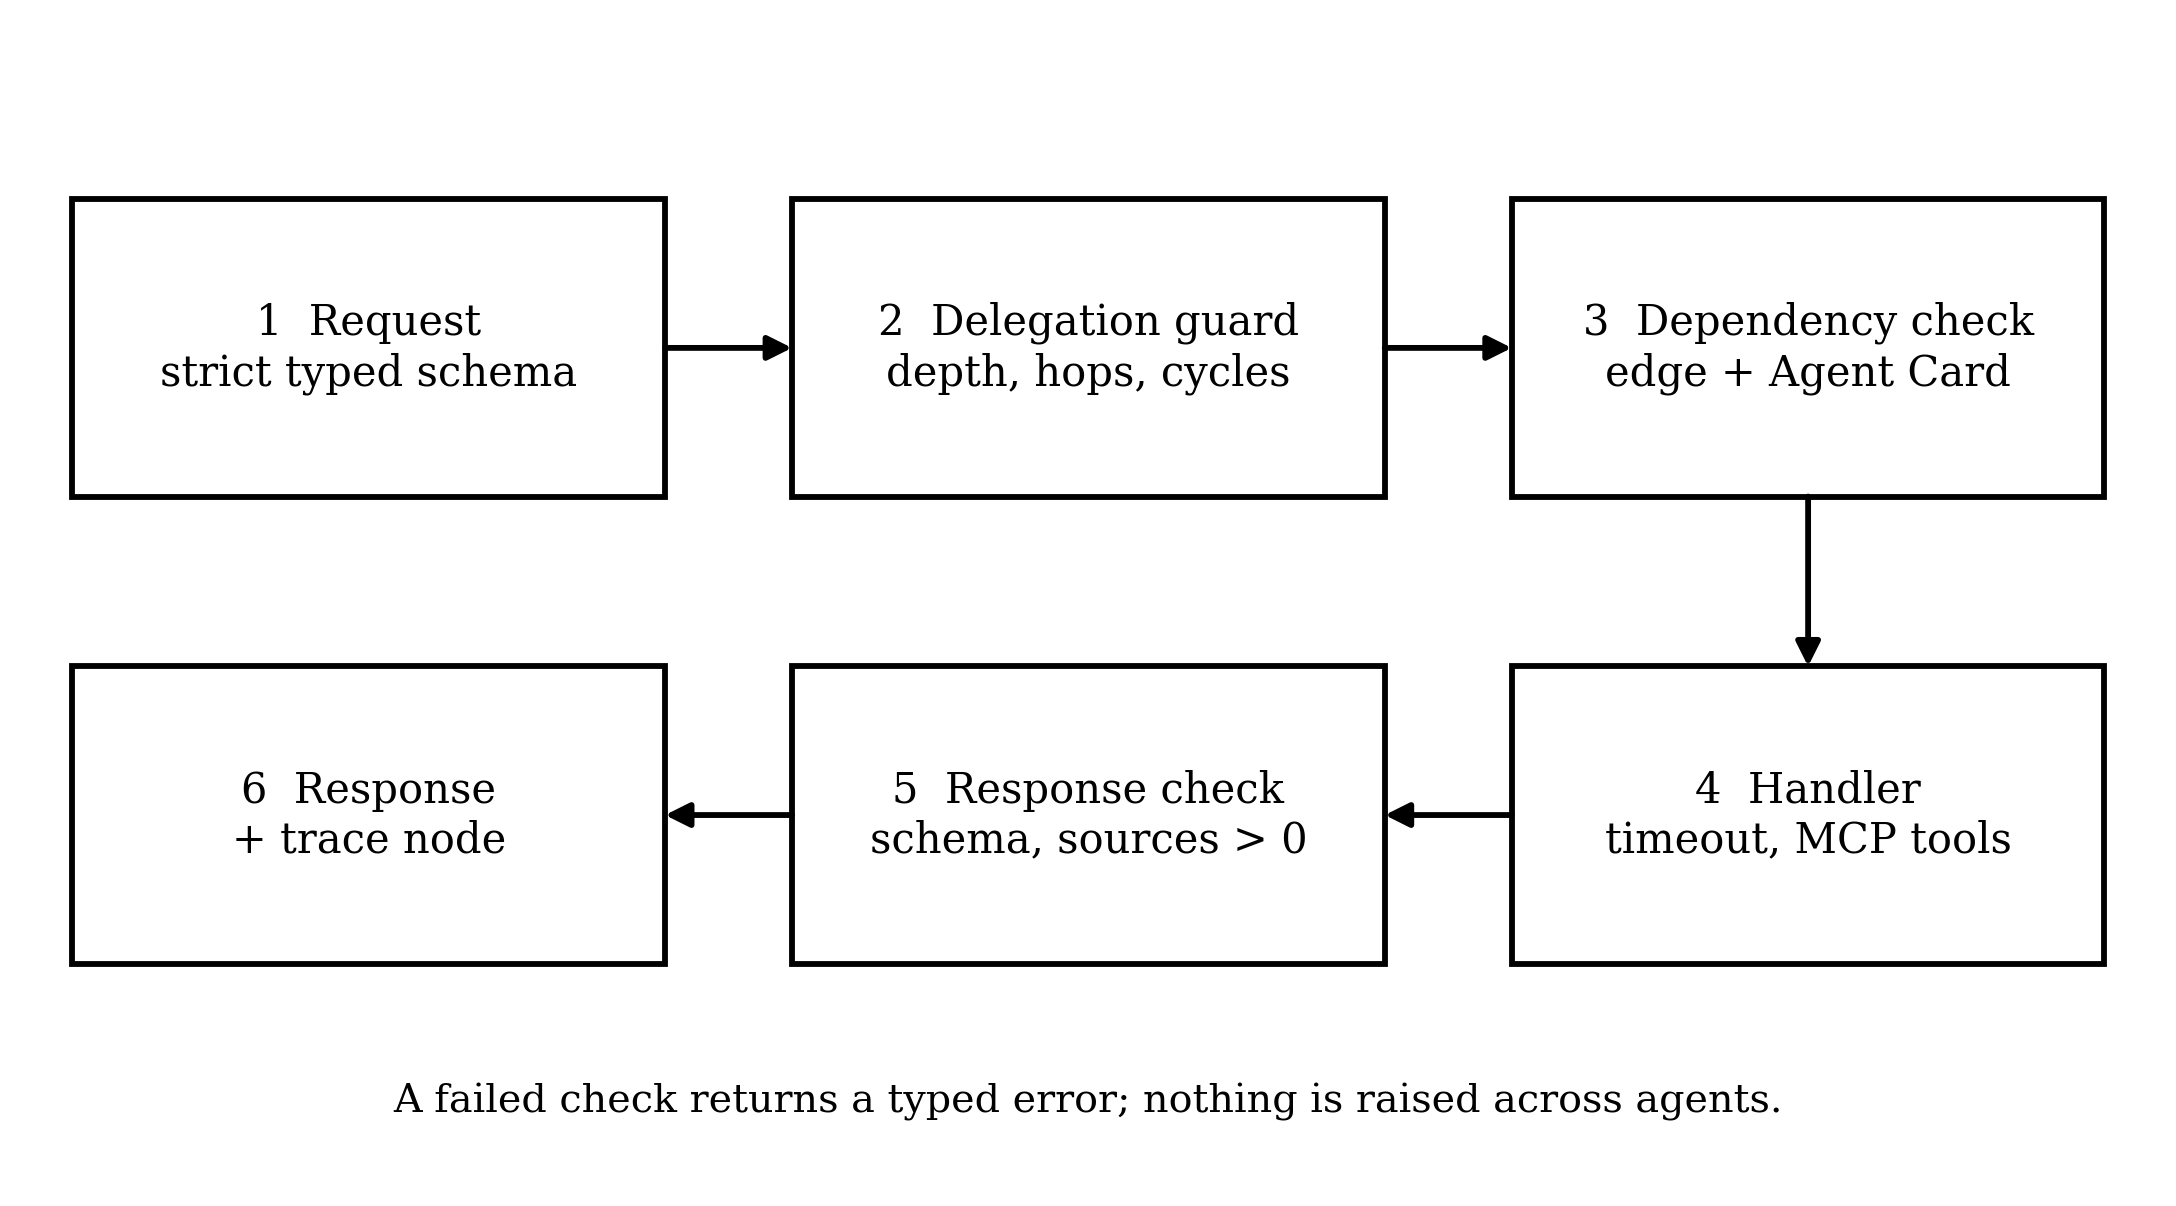
\includegraphics[width=0.78\textwidth]{03_a2a_request_pipeline.png}
\caption{Request handling in the A2A server. Guards run before any handler code. Every rejection is a typed error response; none is raised across agent boundaries.}
\label{fig:a2apipeline}
\end{figure*}

\subsection{Agent Cards and routing}
Each sector agent publishes an Agent Card with a stable identifier, capabilities, skill tags, supported tasks and routing keywords. The orchestrator scores each card against the query. A keyword advertised by $n$ agents contributes $1/n$ to each, so a shared term such as ``RBI'' does not drag unrelated sectors into the answer. Only when no card matches does the system ask an LLM to choose receivers, and its answer is intersected with the registered identifiers. The LLM therefore selects among receivers but cannot bypass delivery through the A2A server.

\subsection{The MCP data plane and provenance}
Each sector owns one FastMCP server that reads official statistical sources (MoSPI, RBI DBIE, Agmarknet, IMD, NSE, CGA and others), DuckDB tables and curated snapshots. Snapshots seeded into the stores are tagged \code{cached} with their publication reference; fixed simulation defaults are tagged \code{DEFAULT} and replaced whenever a live observation exists. \Cref{fig:provenance} follows one value from source to report. The same provenance record travels unchanged through the A2A server and client, so the orchestrator sees the original table, URL and reporting period, not a paraphrase.

\begin{figure}[t]
\centering
% IMAGE 05 -- Provenance chain
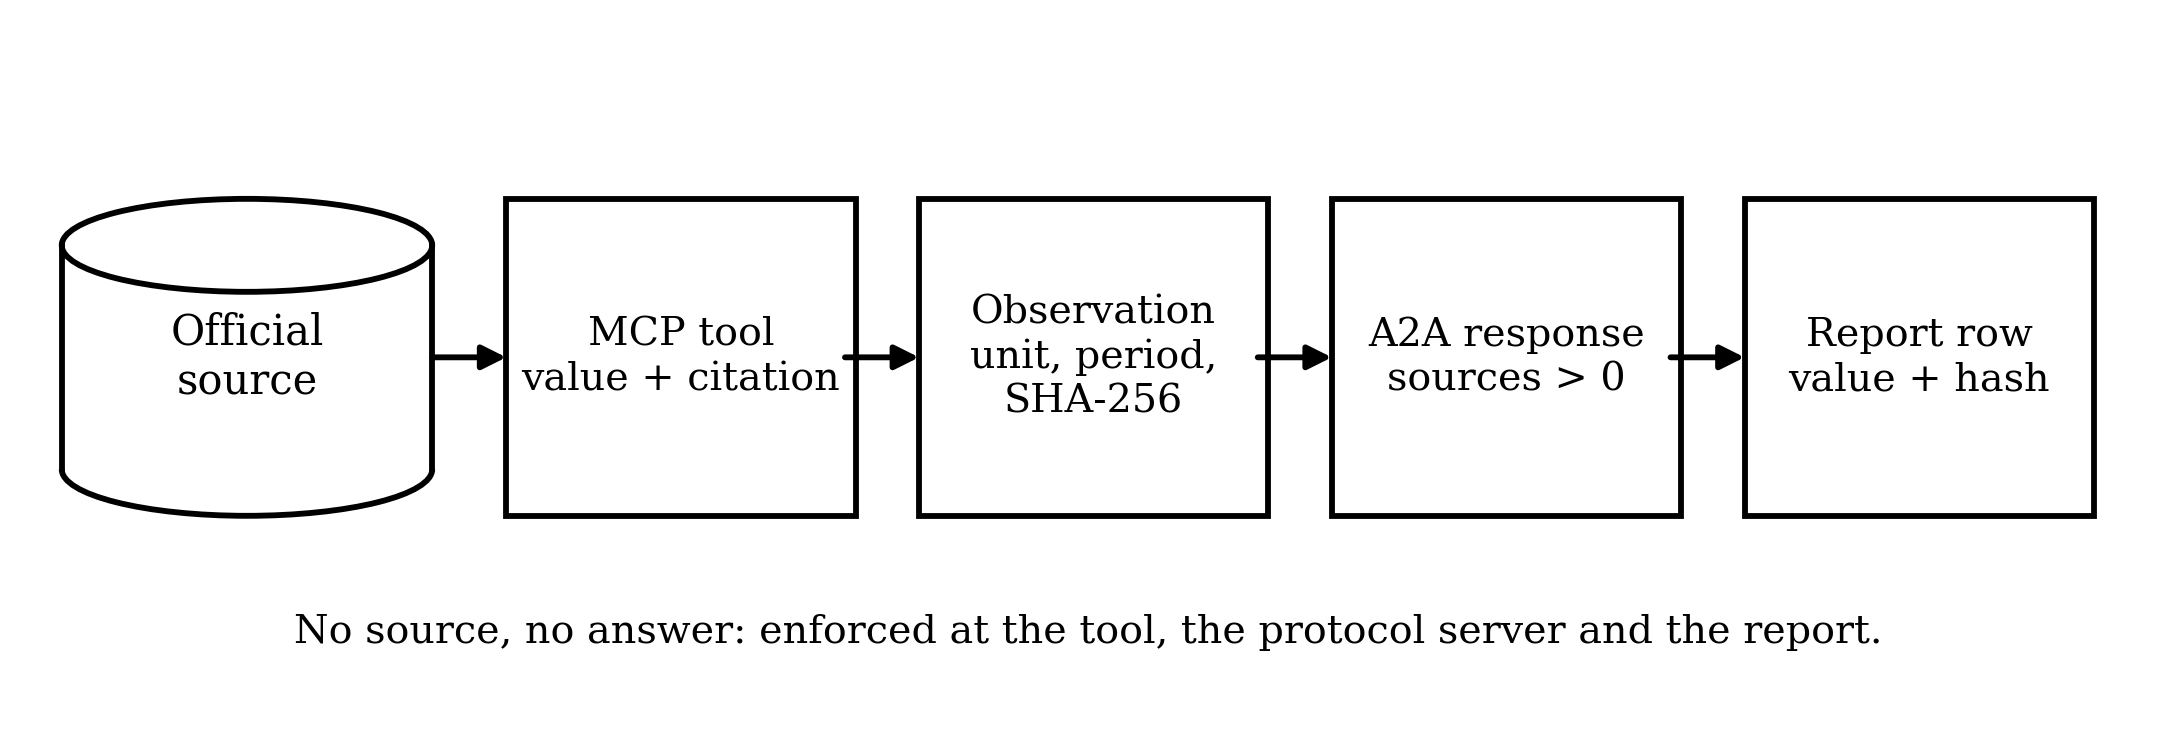
\includegraphics[width=\columnwidth]{05_provenance_chain.png}
\caption{Provenance chain. ``No source, no answer'' is enforced at the tool, at the protocol server and at report rendering.}
\label{fig:provenance}
\end{figure}

\subsection{Orchestration}
The orchestrator is a four-node LangGraph state graph (\cref{fig:orchestrator}). \emph{Decompose} routes the query; \emph{parallel A2A execute} sends one \code{sector_analysis} request per routed agent concurrently and runs at most one bounded follow-up round; \emph{KG causal enrichment} finds transmission paths between the observed indicators and, if the query asks for it, simulates a shock using live observations as baselines; \emph{synthesis} produces a report containing an indicator matrix with provenance hashes, a causal diagram, a path table, a scenario table, a source table and the list of agents that failed to answer. If an agent fails, the run continues with partial data and the failure appears in the report. Without an LLM key every stage falls back to a deterministic summary, which makes the platform testable offline.

\begin{figure*}[t]
\centering
% IMAGE 04 -- Orchestrator pipeline
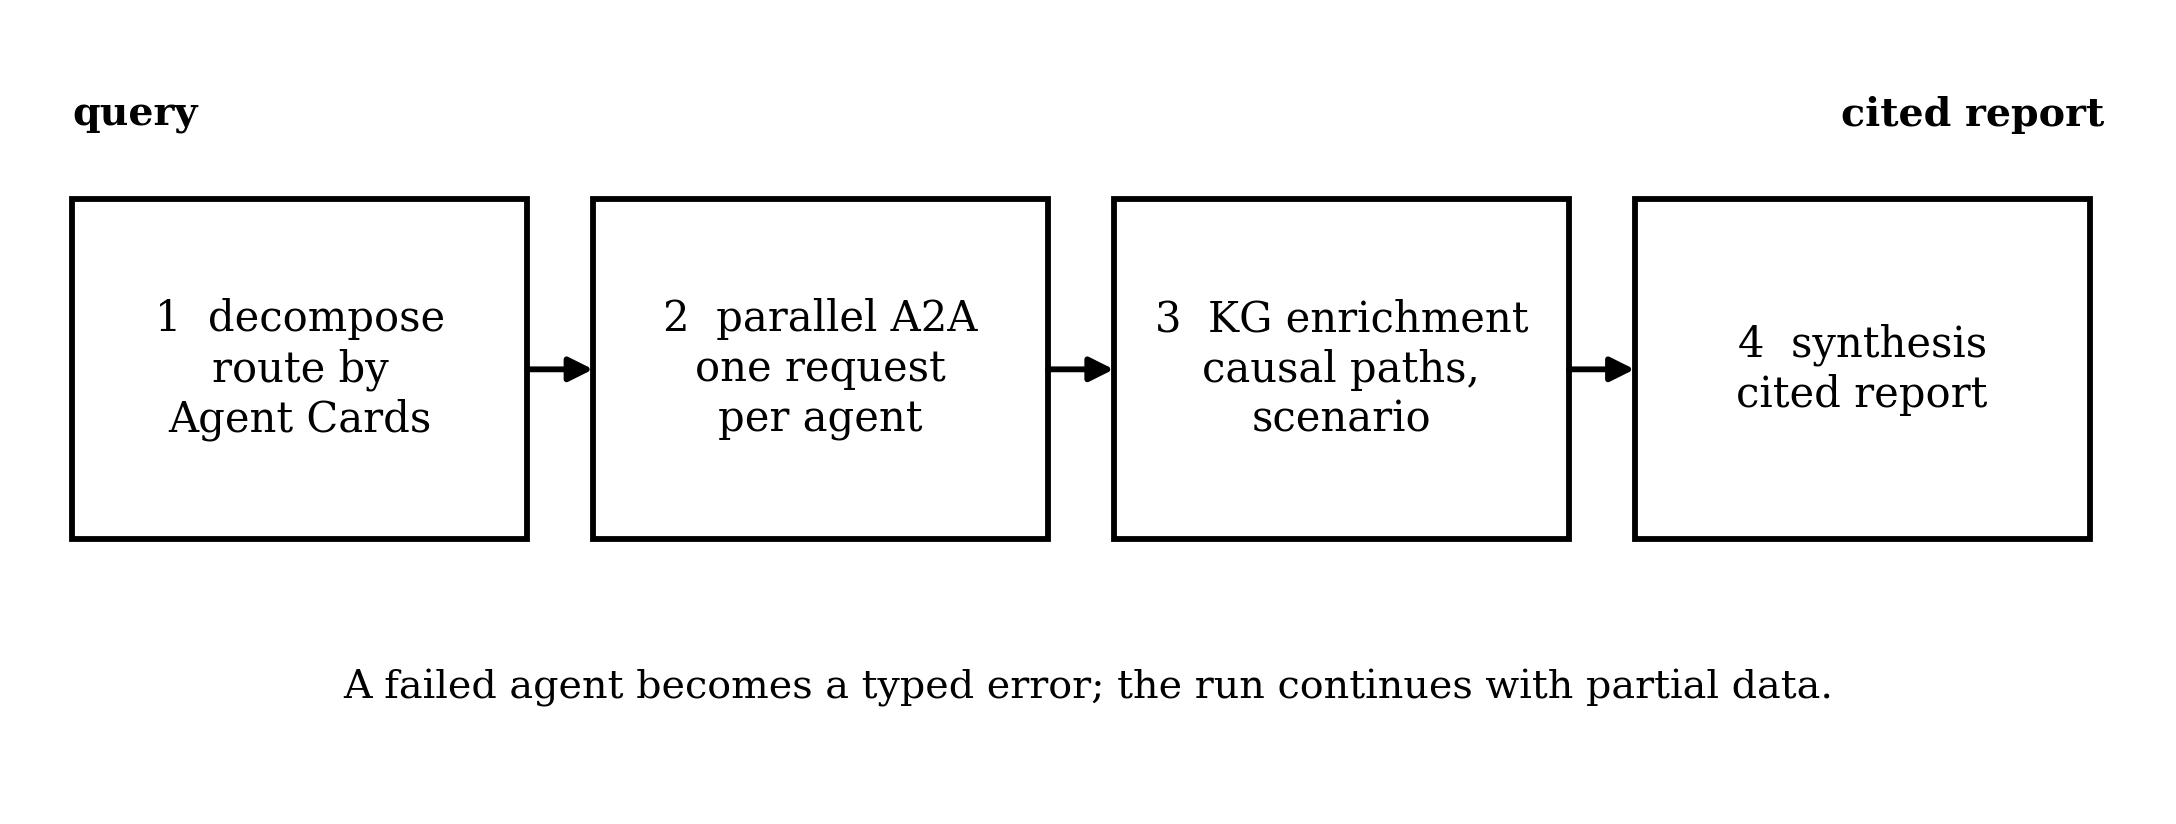
\includegraphics[width=0.9\textwidth]{04_orchestrator_pipeline.png}
\caption{The four-node orchestrator. Failures become typed errors in the state and the run continues with partial data.}
\label{fig:orchestrator}
\end{figure*}

% ================================================================ IV. KG
\section{Evidence-Graded Causal Knowledge Graph}
\label{sec:kg}

\subsection{Ontology and edge schema}
The ontology contains 20 canonical indicators across eight domains (real, prices, monetary, fiscal, external, capital markets, agriculture, labour) and 12 directed causal relations (\cref{fig:kg}). Each indicator has a canonical identifier of the form \code{in.macro.<domain>.<name>}, a unit, a frequency and a source authority. Each relation is a record with a source and target indicator, a relation type from the five-tier taxonomy, a transmission lag in months, an elasticity sign, an empirical $p$-value, a confidence score, a mechanism description and documented assumptions. Relation identifiers are deterministic: $\textsf{rel-}h$, where $h$ is the first eight hexadecimal characters of a version-5 UUID computed over the string \code{source|target|type}. This keeps identifiers stable across restarts so they can serve as provenance keys and as merge keys for the optional Neo4j mirror. A validator rejects self-loops, unknown endpoints and duplicate identifiers before the graph is built.

\begin{figure*}[t]
\centering
% IMAGE 06 -- Causal knowledge graph
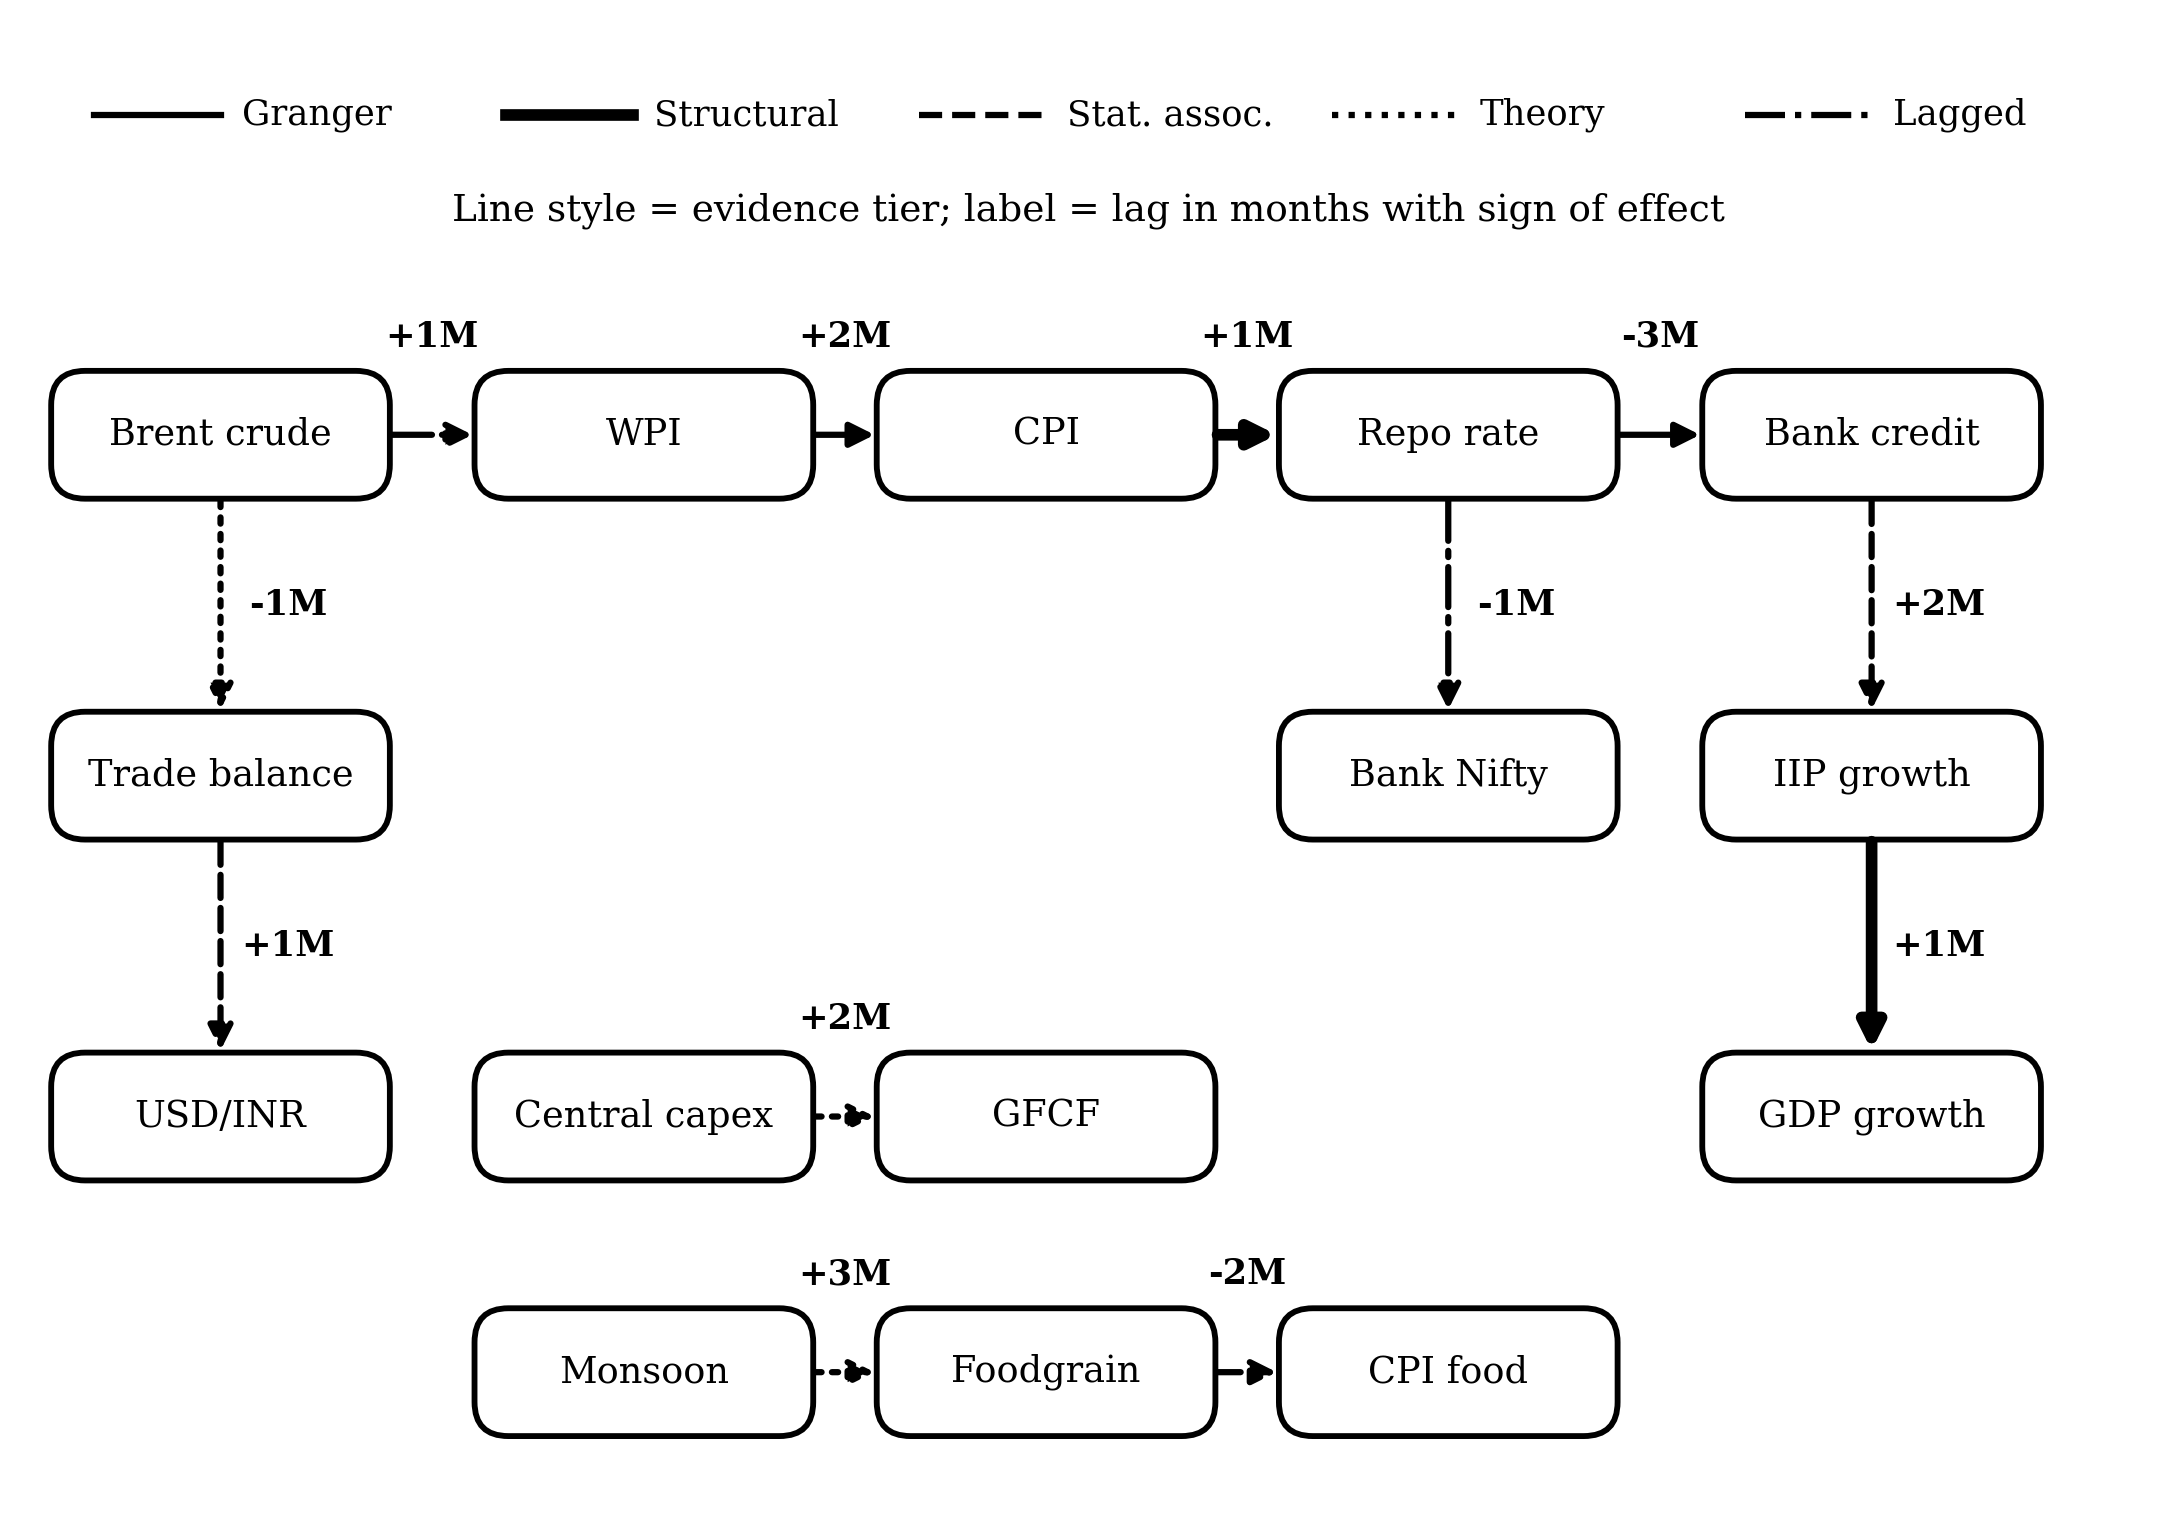
\includegraphics[width=0.88\textwidth]{06_causal_knowledge_graph.png}
\caption{The causal knowledge graph: 20 indicators (15 shown on the connected transmission chains) and 12 edges. Line style encodes the evidence tier of the edge (see legend); labels give the lag in months with the sign of the effect. The canonical chain is Brent $\rightarrow$ WPI $\rightarrow$ CPI $\rightarrow$ repo $\rightarrow$ credit $\rightarrow$ IIP $\rightarrow$ GDP (10 months in total).}
\label{fig:kg}
\end{figure*}

\subsection{Five-tier taxonomy}
The tiers rise from qualitative theory to an identified structural model: \textsc{Theory}, \textsc{Statistical association}, \textsc{Lagged relationship}, \textsc{Granger predictive} and \textsc{Structural causal model}. The current ontology has three, three, two, two and two edges respectively (\cref{tab:edges}). The tier is assigned by hand at present, and a tier name is a claim. We therefore do not read the assigned tier as evidence. The audit below tests it.

\begin{table}[t]
\centering
\caption{The 12 transmission edges. Conf.\ is the seeded confidence score; Audit is the audit status on the bundled data (\code{N}: fewer than 10 overlapping months; \code{D}: no data).}
\label{tab:edges}
\footnotesize
\setlength{\tabcolsep}{3.2pt}
\begin{tabular}{@{}llcrcc@{}}
\toprule
\textbf{Edge} & \textbf{Tier} & \textbf{Sign} & \textbf{Lag} & \textbf{Conf.} & \textbf{Audit} \\
\midrule
Brent $\to$ WPI & Lagged & $+$ & 1 & 0.95 & N \\
WPI $\to$ CPI & Granger & $+$ & 2 & 0.90 & N \\
CPI $\to$ Repo & Structural & $+$ & 1 & 0.95 & N \\
Repo $\to$ Credit & Granger & $-$ & 3 & 0.88 & D \\
Credit $\to$ IIP & Stat.\ assoc. & $+$ & 2 & 0.82 & D \\
IIP $\to$ GDP & Structural & $+$ & 1 & 0.98 & D \\
Brent $\to$ Trade bal. & Theory & $-$ & 1 & 0.92 & N \\
Trade bal. $\to$ USD/INR & Stat.\ assoc. & $+$ & 1 & 0.86 & N \\
Repo $\to$ Bank Nifty & Lagged & $-$ & 1 & 0.85 & D \\
Capex $\to$ GFCF & Theory & $+$ & 2 & 0.90 & D \\
Monsoon $\to$ Foodgrain & Theory & $+$ & 3 & 0.92 & D \\
Foodgrain $\to$ CPI food & Stat.\ assoc. & $-$ & 2 & 0.89 & D \\
\bottomrule
\end{tabular}
\end{table}

\subsection{Graph queries}
A NetworkX multi-digraph is built from the ontology (with an optional Neo4j mirror). Three queries serve the rest of the system: the shortest transmission path between two indicators, the set of downstream impacts of an indicator with the cumulative lag (sum of edge lags) and cumulative confidence (product of edge confidences), and a causal neighbourhood. For a path $P=(e_1,\dots,e_k)$,
\begin{equation}
L(P)=\sum_{i=1}^{k}\ell_{e_i},\qquad C(P)=\prod_{i=1}^{k}c_{e_i},
\label{eq:pathlagconf}
\end{equation}
where $\ell_e$ is the lag in months and $c_e$ the edge confidence.

\subsection{Edge Evidence Audit}
Hand-assigned $p$-values and confidences are the weakest part of any curated graph, because they look like measurements. The Edge Evidence Audit separates what was typed from what was tested. For each edge $e=(u\to v)$ it aligns the two monthly series from the platform's cached telemetry, and
\begin{enumerate}
\item reports \code{UNTESTABLE_NO_DATA} if either series is absent;
\item reports \code{UNTESTABLE_N} if the overlap has fewer than $n_{\min}=10$ months;
\item otherwise runs a bivariate Granger test with lags $1,\dots,L$ and records
\begin{equation}
p_e=\min_{1\le \ell\le L} p^{F}_{\ell},\qquad \text{significant}\iff p_e<0.05,
\label{eq:granger}
\end{equation}
where $p^{F}_{\ell}$ is the $p$-value of the sum-of-squared-residuals $F$ test at lag $\ell$, and labels the edge \code{EMPIRICAL}.
\end{enumerate}
Every edge not labelled \code{EMPIRICAL} is shown as \code{SEEDED} wherever it appears: on the graph, in the Twin comparison and in the model card of a chat answer. One edge also carries a manual review note. The edge from the trade balance to USD/INR has a positive sign, but its documented mechanism (a wider deficit weakens the rupee) implies that the \emph{USD/INR rate rises} when the balance falls, which is a negative sign if the balance is defined as exports minus imports. We keep the defect visible instead of hiding it (\cref{sec:discussion}).

\textbf{Result on the bundled data.} \Cref{fig:audit} shows the outcome. All 12 edges are untestable: five have some overlap but far fewer than ten months, and seven have no usable series at all. The practical consequence is that every causal statement the system produces today is \code{SEEDED}, and the system says so. We consider this a finding rather than a failure. It shows quantitatively how thin the machine-readable history behind a typical ``causal graph'' is, and it identifies the data work (long monthly back-series from RBI DBIE and MoSPI) that must precede any claim of empirical support. The audit procedure also has known weaknesses that we list in \cref{sec:discussion} (no stationarity check, no multiplicity correction, a minimum over lags that inflates false positives).

\begin{figure}[t]
\centering
% IMAGE 08 -- Edge evidence audit result
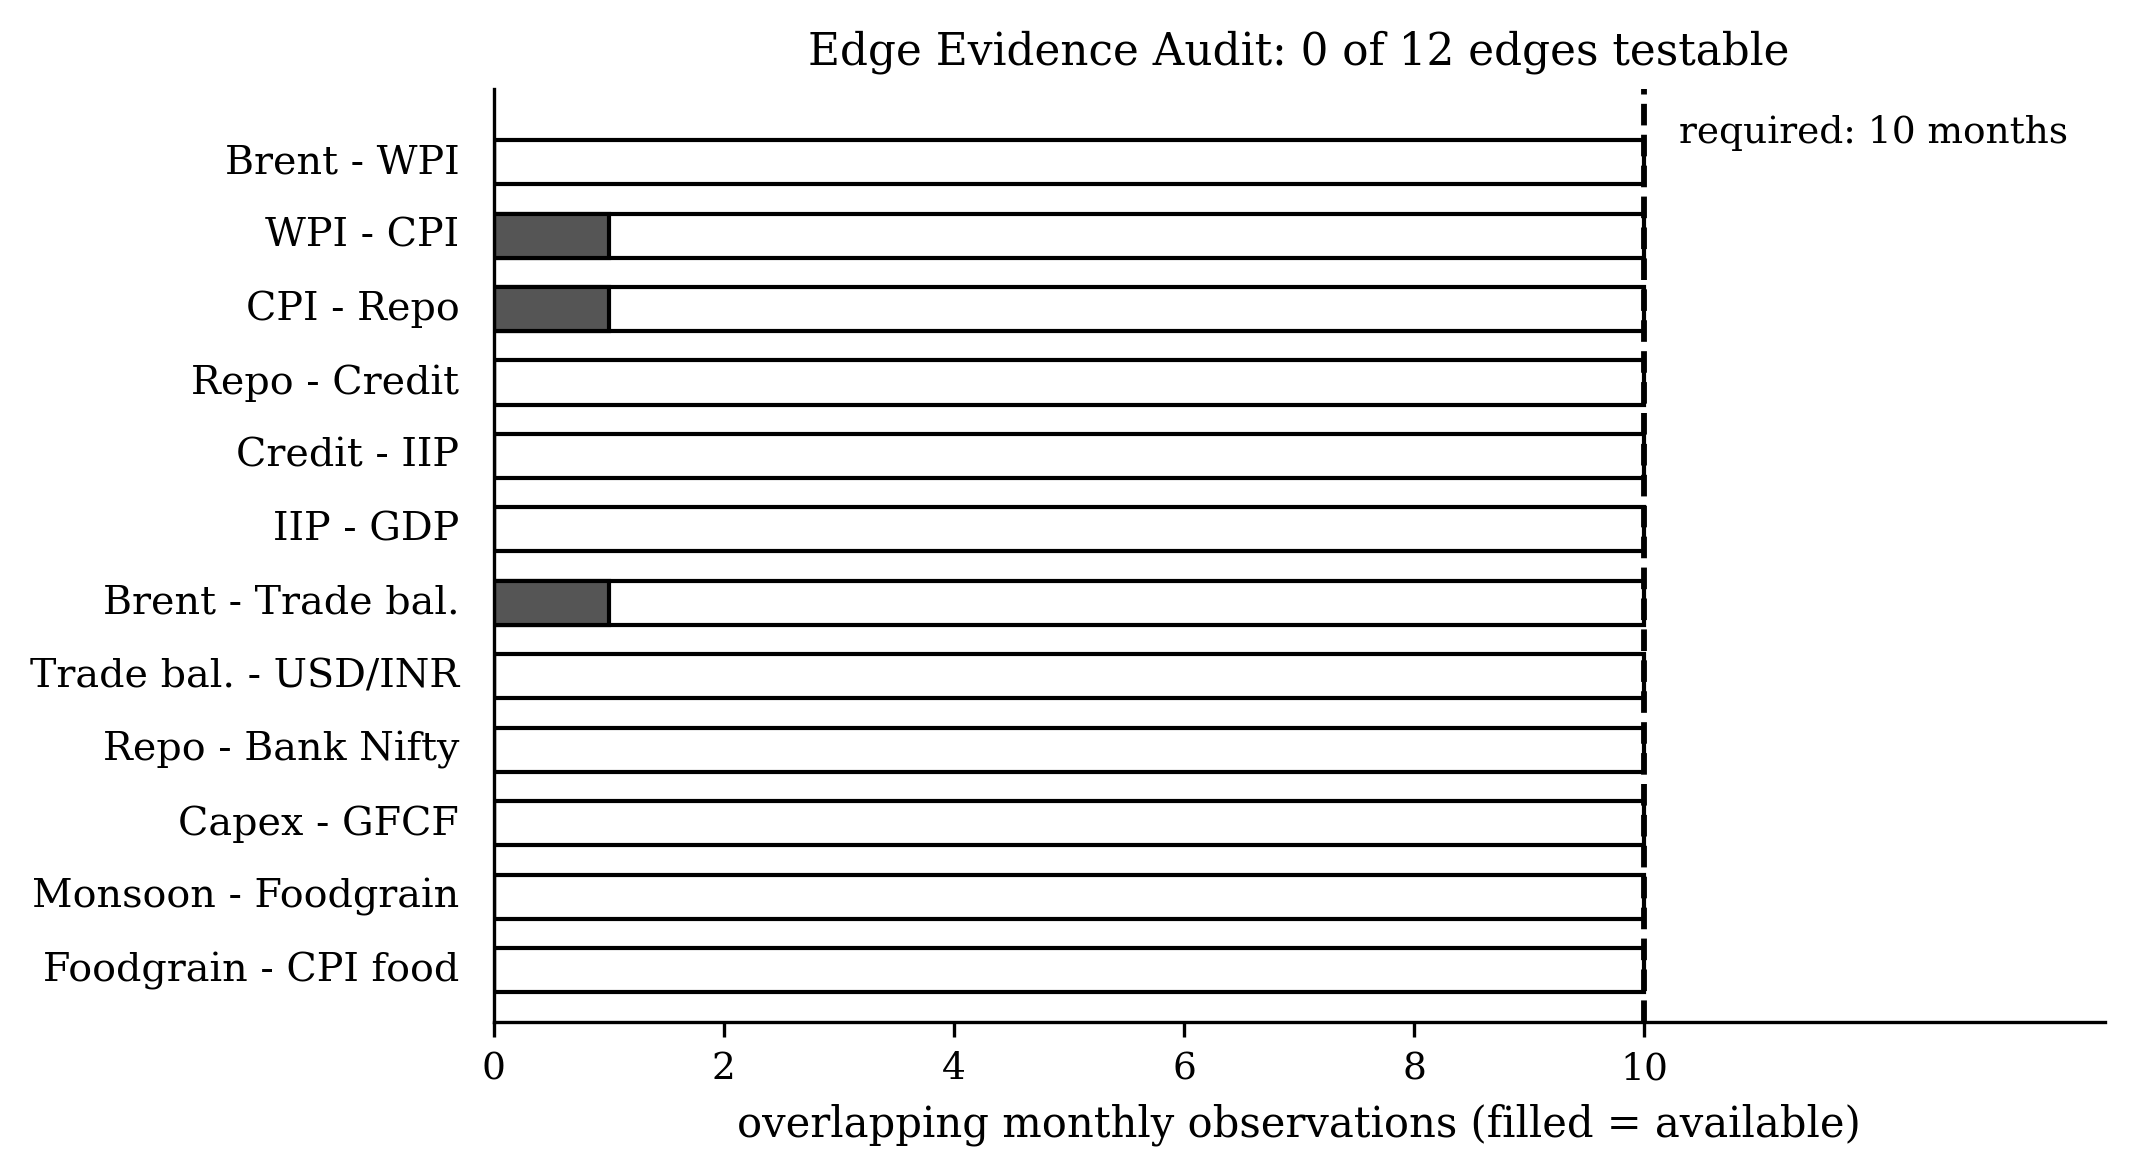
\includegraphics[width=\columnwidth]{08_edge_evidence_audit.png}
\caption{Edge Evidence Audit on the bundled data. Filled bars show the overlapping monthly observations that exist; the dashed line is the 10-month minimum. None of the 12 edges can be tested, so all remain \code{SEEDED}.}
\label{fig:audit}
\end{figure}

% ================================================================ V. scenario
\section{Scenario Engine}
\label{sec:scenario}

\subsection{Model}
Given a shock of size $s$ (in the unit of the source indicator $i$), the engine finds the shortest transmission path $P_{i\to j}$ to each downstream indicator $j$ and computes
\begin{equation}
\Delta_j \;=\; \gamma\, s \prod_{e\in P_{i\to j}} \sigma_e\,\alpha\, c_e ,
\qquad \alpha=0.55,\ \gamma=0.15,
\label{eq:scenario}
\end{equation}
where $\sigma_e\in\{+1,-1\}$ is the sign of edge $e$ and $c_e$ its confidence. The shocked value is $x_j+\Delta_j$, where $x_j$ is the baseline (the latest live observation when the owner agent supplied one, otherwise a labelled default), and the reported band is $x_j+\Delta_j\pm 0.25\,|\Delta_j|$. \Cref{alg:scenario} lists the procedure.

\begin{algorithm}[t]
\caption{Graph-attenuation scenario propagation}
\label{alg:scenario}
\begin{algorithmic}[1]
\Require shock indicator $i$, magnitude $s$, baselines $B$ (live where available)
\Ensure impacts $\{(j,\Delta_j,\text{band},L_j,C_j)\}$ and the list of traversed relation ids
\State $\mathcal{D}\gets$ downstream impacts of $i$ in the graph
\For{each $j\in\mathcal{D}$}
  \State $P\gets$ shortest transmission path $i\to j$
  \State $m\gets 1$
  \For{each edge $e\in P$}
     \State $m\gets m\cdot \sigma_e\cdot 0.55\cdot c_e$; record relation id of $e$
  \EndFor
  \State $\Delta_j\gets 0.15\cdot s\cdot m$
  \State band$_j\gets [\,B_j+\Delta_j-0.25|\Delta_j|,\; B_j+\Delta_j+0.25|\Delta_j|\,]$
\EndFor
\State \Return impacts and de-duplicated relation ids
\end{algorithmic}
\end{algorithm}

\subsection{What the model is, and is not}
The model is a deterministic, closed-form attenuation rule. It is easy to inspect, it has no free parameters beyond two documented constants, and its output can be reproduced by hand. It is \emph{not} an identified econometric model. In particular: (i) the constants $\alpha$ and $\gamma$ are not estimated; (ii) the same scaling is applied to every target regardless of its unit, so a shock in USD per barrel is mapped into percentage points of CPI and into index points of Bank Nifty without a unit conversion; (iii) the $\pm25\%$ band is a fixed fraction of $\Delta_j$, not a confidence interval; and (iv) the horizon argument does not enter the arithmetic. The user interface and the model card say ``graph-attenuation, heuristic'' for these reasons, and we recommend citing the engine only as a named baseline against which a local-projection or vector-autoregression estimator should be compared \cite{jorda2005lp,sims1980macro}.

\subsection{Worked example}
\Cref{tab:brent} and \cref{fig:brent} show a \$20 per barrel increase in Brent crude with the default baselines, which we obtained by running the engine on the released code. The shock reaches WPI after one month and GDP after ten. Confidence falls from 0.95 to 0.57 along the chain, and the effect on each successive indicator shrinks by roughly a factor of two per hop in magnitude (per unit of shock, $|\Delta_j|/s$ falls from $7.9\times10^{-2}$ at WPI to $2.5\times10^{-3}$ at GDP). The sign of the effect on credit growth is negative because the repo-to-credit edge is negative. The model also reports USD/INR \emph{falling} by 0.72 after an oil price rise. That is the sign defect described above, and it is the reason the user interface marks the edge with a warning and the reason we advise against quoting this particular row.

\begin{table}[t]
\centering
\caption{Simulated effect of Brent $+\$20$/bbl (default baselines). $\Delta$ is in the target's own unit; Lag is the cumulative transmission lag in months; Conf.\ is the cumulative path confidence $C(P)$.}
\label{tab:brent}
\footnotesize
\setlength{\tabcolsep}{4pt}
\begin{tabular}{@{}lrrrr@{}}
\toprule
\textbf{Indicator} & \textbf{Baseline} & \textbf{$\Delta$} & \textbf{Lag} & \textbf{Conf.} \\
\midrule
WPI inflation (\% YoY) & 2.45 & $+1.57$ & 1 & 0.95 \\
Trade balance (\$bn) & $-22.50$ & $-1.52$ & 1 & 0.92 \\
CPI headline (\% YoY) & 4.26 & $+0.78$ & 3 & 0.85 \\
USD/INR$^{\dagger}$ & 86.40 & $-0.72$ & 2 & 0.79 \\
Repo rate (\%) & 6.25 & $+0.41$ & 4 & 0.81 \\
Bank Nifty (points) & 51{,}500 & $-0.19$ & 5 & 0.69 \\
Bank credit growth (\%) & 13.80 & $-0.20$ & 7 & 0.71 \\
IIP growth (\%) & 4.20 & $-0.09$ & 9 & 0.59 \\
GDP growth (\%) & 5.40 & $-0.05$ & 10 & 0.57 \\
\bottomrule
\multicolumn{5}{@{}l}{\scriptsize $^{\dagger}$Sign under review; see \cref{sec:kg}.}
\end{tabular}
\end{table}

\begin{figure}[t]
\centering
% IMAGE 07 -- Brent scenario results
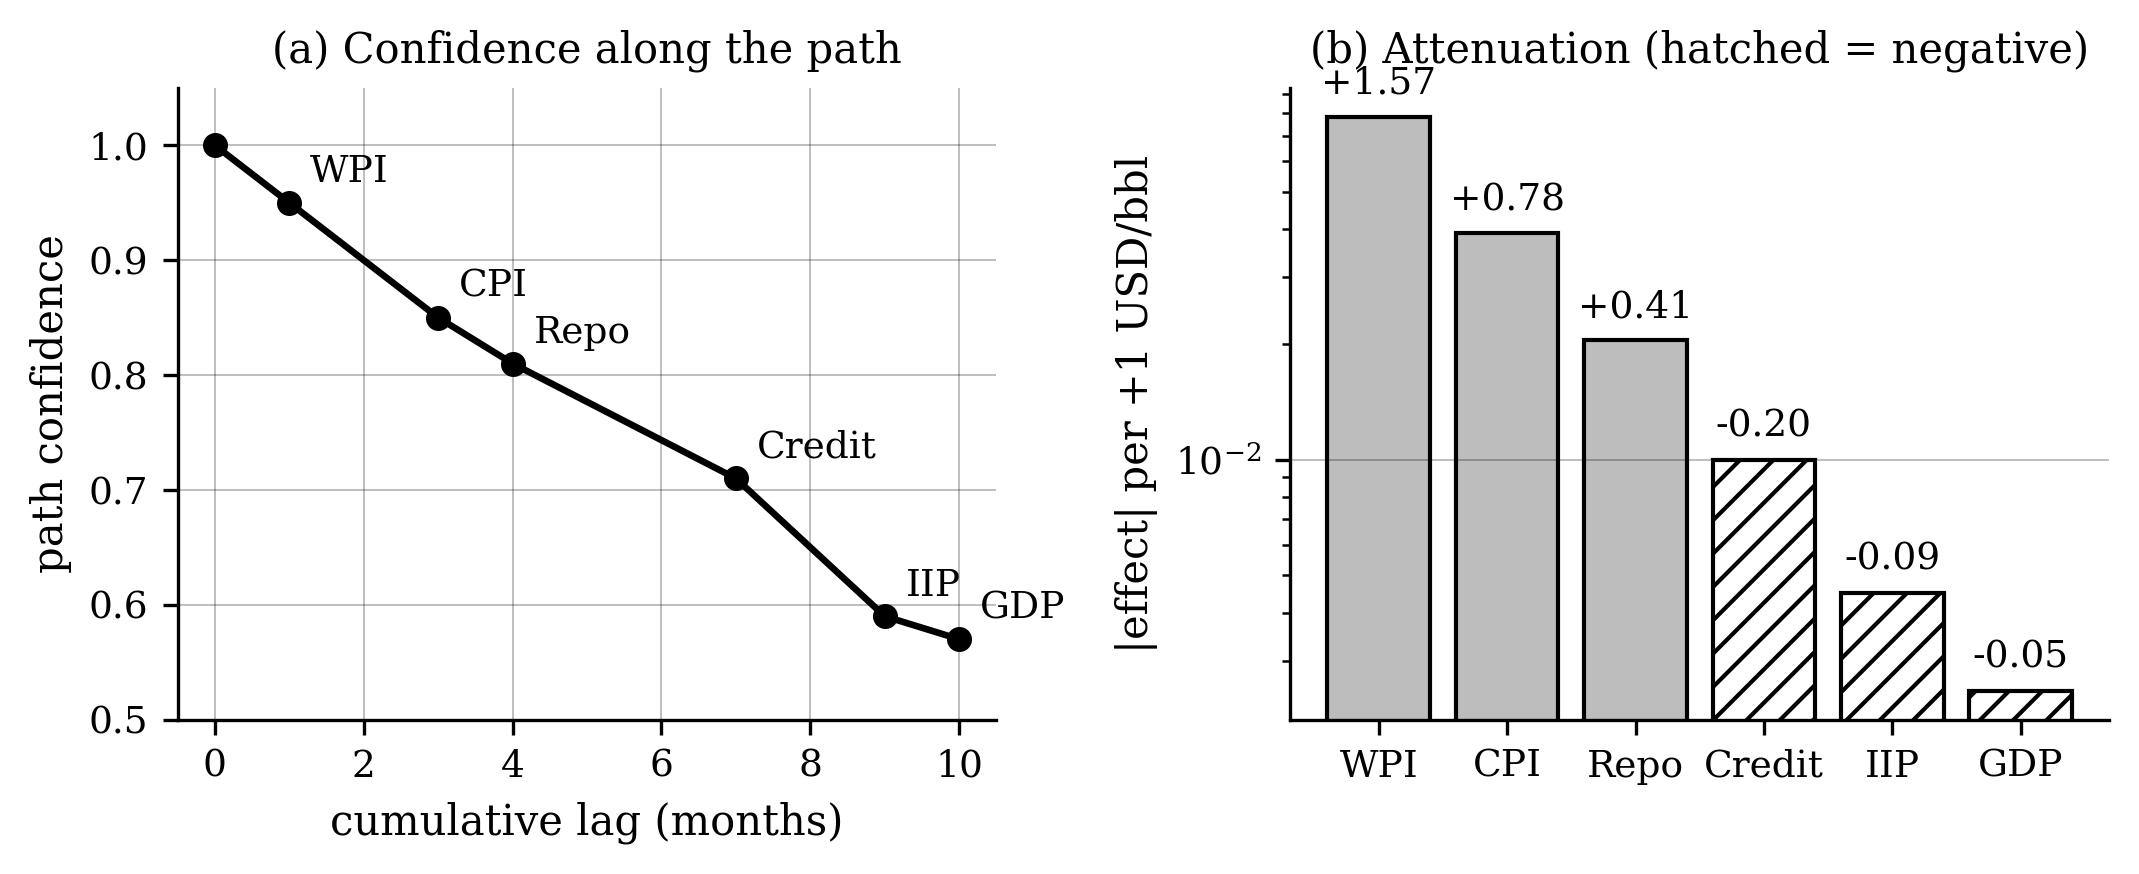
\includegraphics[width=\columnwidth]{07_brent_scenario_results.png}
\caption{Brent $+\$20$/bbl. (a) Cumulative path confidence by transmission lag. (b) Magnitude of the effect per unit of shock on a logarithmic axis (hatched bars are negative effects); labels give the simulated change in the indicator's own unit.}
\label{fig:brent}
\end{figure}

% ================================================================ VI. lab
\section{Research Lab}
\label{sec:lab}

The research lab is a set of pure functions over the frozen outputs of the engine, the graph and the trace store (\cref{fig:lab}). It never mutates engine state, and its extras are best-effort: if one fails, the primary answer is unaffected. Every output carries a data-status label.

\begin{figure}[t]
\centering
% IMAGE 10 -- Research lab modules
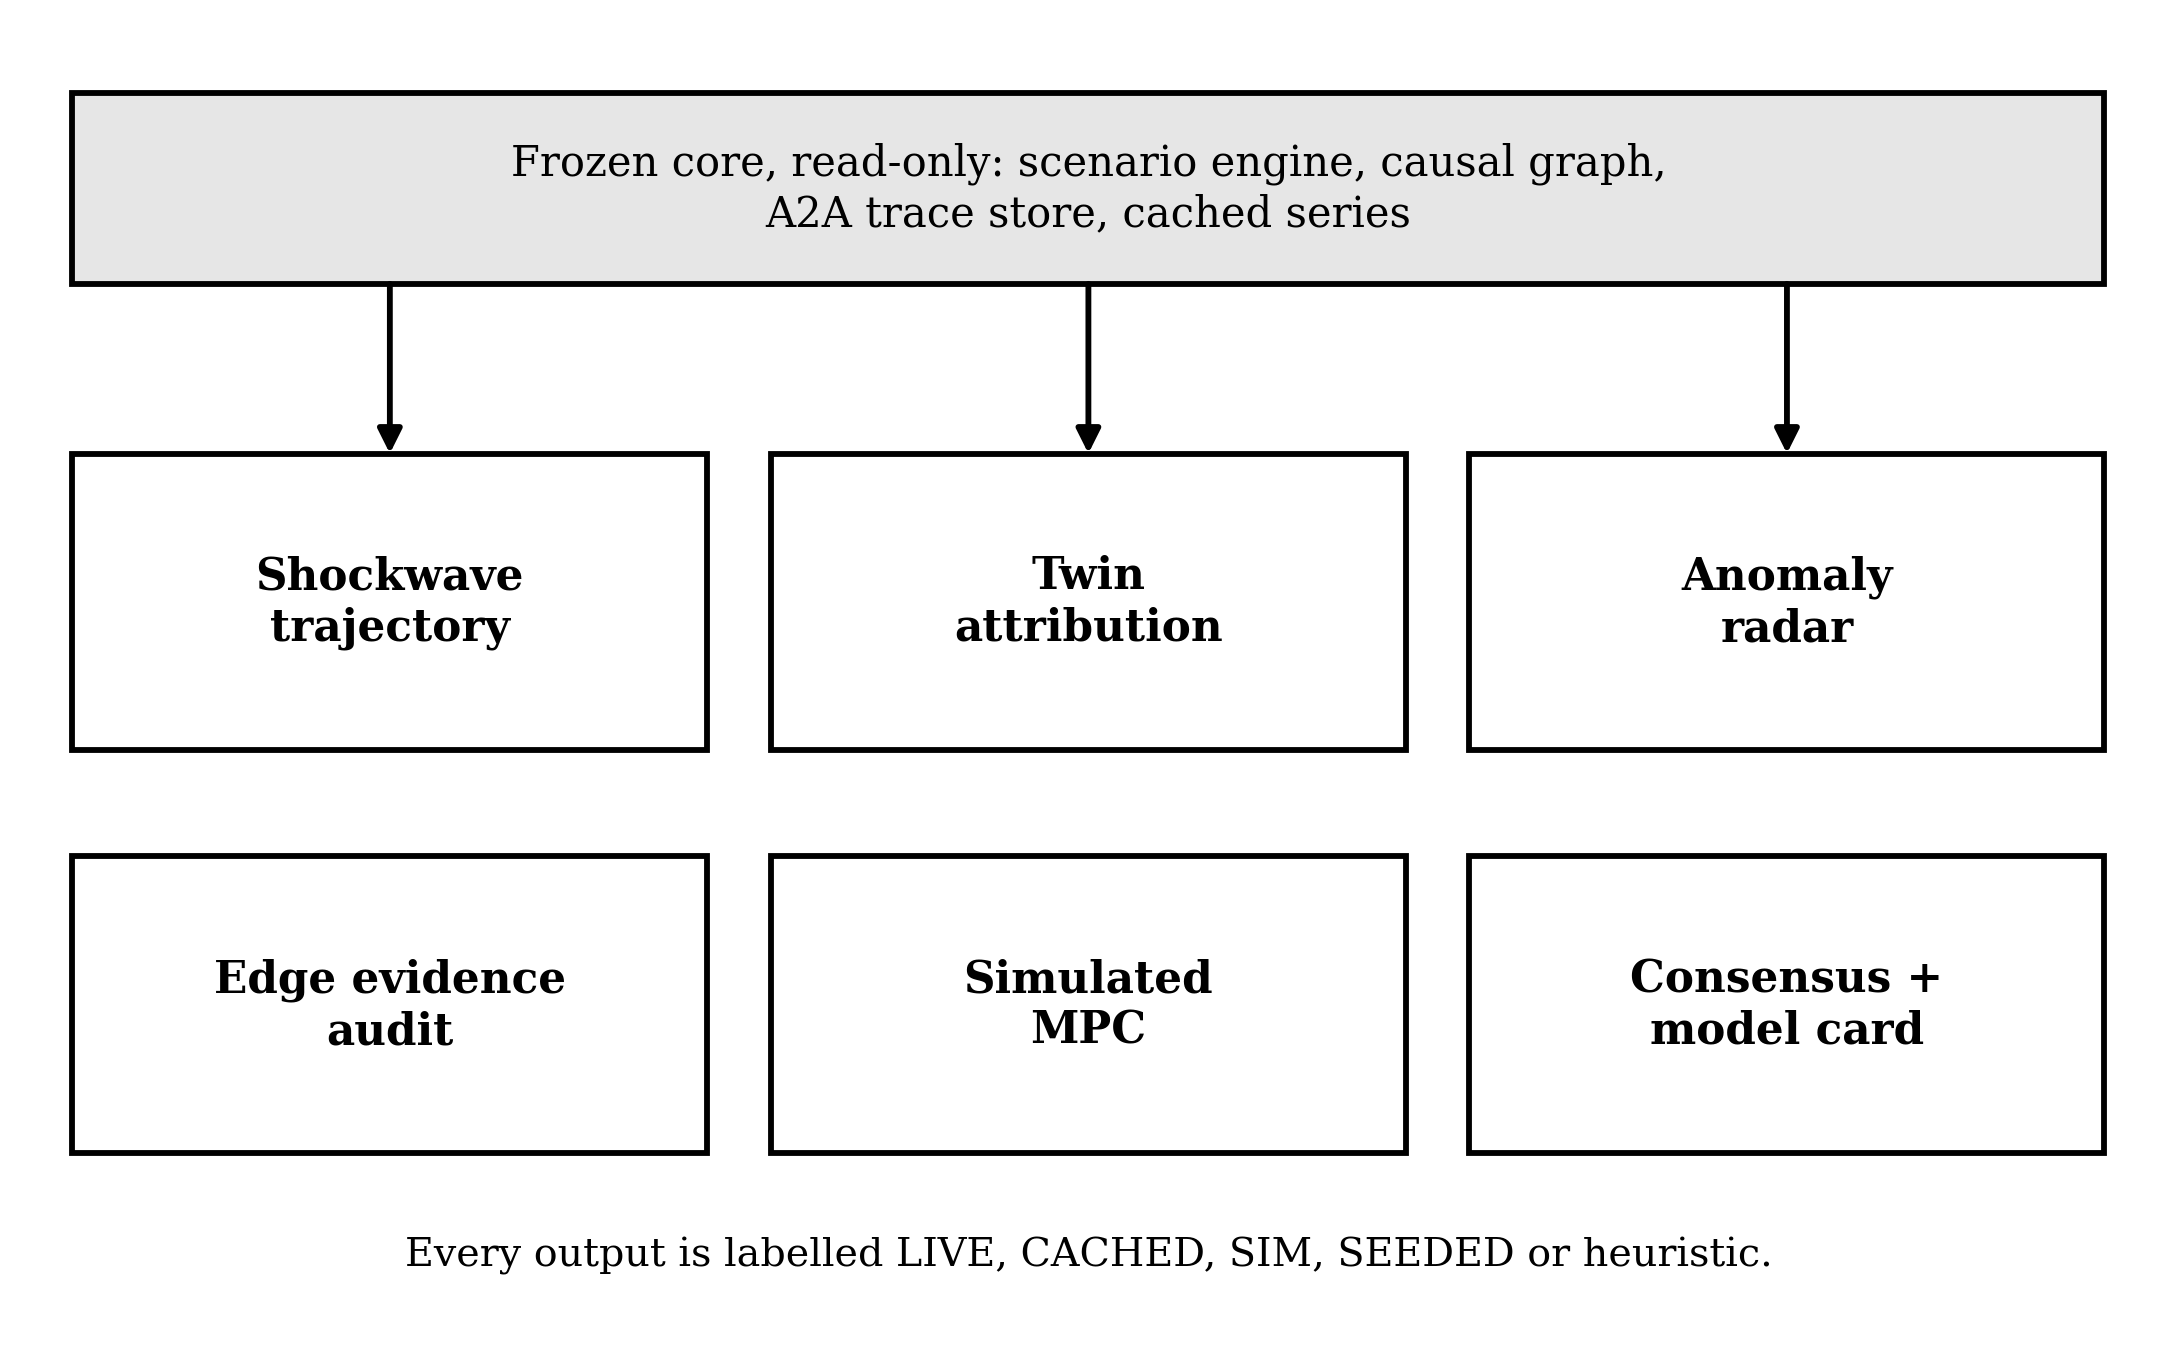
\includegraphics[width=\columnwidth]{10_research_lab_modules.png}
\caption{Research-lab modules. All read frozen core components and label their output.}
\label{fig:lab}
\end{figure}

\paragraph{Shockwave trajectory.}
The one-shot scenario result is expanded into a monthly series per node. With lag $\ell_j$ and horizon $H$, the \emph{step} shape is $x_j(t)=B_j$ for $t<\ell_j$ and $B_j+\Delta_j$ afterwards. The optional \emph{decay} shape multiplies $\Delta_j$ by $2^{-(t-\ell_j)/h}$ for half-life $h$. The decay shape is a drawing choice for illustration, not a fitted dynamic.

\paragraph{Twin attribution.}
The twin compares a base world ($s=0$) with the shocked world and attributes the attenuation along a path to its edges. With per-edge gain $g_e=\alpha c_e$, the share of edge $e$ is
\begin{equation}
\phi_e=\frac{\ln g_e}{\sum_{e'\in P}\ln g_{e'}},\qquad \sum_{e\in P}\phi_e=1 ,
\label{eq:attrib}
\end{equation}
and the edge with the largest share is reported as the weakest link. The share reflects how much the \emph{edge confidence} weakens the signal, and it should not be read as an estimated causal contribution.

\paragraph{Anomaly radar.}
For each series with at least $N_{\min}=8$ points, the latest value is compared with the preceding window of $w=\min(12,n-1)$ points:
\begin{equation}
z_t=\frac{x_t-\mu_{t-1}^{(w)}}{\sigma_{t-1}^{(w)}},
\label{eq:z}
\end{equation}
and the series is flagged when $|z_t|>2$. A flagged indicator is then classified against its graph neighbours: \textsc{Propagating} if at least one neighbour with data is also anomalous (with a score equal to the anomalous share), \textsc{Isolated} if neighbours have data but none is anomalous, and \textsc{Unlinked} if there is no neighbour with data. Series that are too short or have zero variance are reported as skipped and never imputed.

\paragraph{Simulated monetary policy committee.}
Six seats are filled by three archetype personas (hawk, dove, centrist) over an evidence pack of CPI, repo rate, GDP growth, USD/INR and credit growth. A deterministic rule engine produces a vote for every persona. The rule thresholds are the inflation-targeting band (2\%, 4\% midpoint, 6\%) in India's monetary policy framework. When an LLM key is available, the model only rewrites the vote and reason for each persona, and the output is accepted only if the vote is valid and the cited indicator belongs to the evidence pack; otherwise the rule vote stands. The result is labelled \code{SIMULATED}. Two caveats are important. The three LLM calls serve six seats, so seats with the same persona vote identically: it is three voices, not six independent members. And the evidence pack uses the latest values, not the vintage at a past meeting date, so the simulator cannot yet be back-tested without look-ahead.

\paragraph{Consensus and model card.}
Each orchestrator answer is accompanied by a heuristic rollup. With $A$ the mean agent success (success $=1$, partial $=0.5$, otherwise $0$), $E$ the share of observations with usable data, $K$ the share of indicator pairs connected by a returned causal path and $\bar c$ the mean confidence of the edges used,
\begin{align}
Q &= A\cdot E\cdot(0.5+0.5\,K), \label{eq:consensus}\\
T &= 0.4\,E + 0.3\,\bar c + 0.3\,A. \label{eq:trust}
\end{align}
Both scores are labelled \code{heuristic}. They are products and weighted sums of fractions with arbitrary weights, not calibrated probabilities. We include them to expose the inputs (evidence cover, edge confidence, agent success) in one place, and we recommend calibrating them against verification outcomes or removing them (\cref{sec:discussion}).

\paragraph{Daily brief.}
A scheduled job combines telemetry, an anomaly scan and cached news into a short brief with one LLM call and a deterministic fallback. History is stored in DuckDB and an optional 08:15 IST schedule can be enabled.

% ================================================================ VII. verify
\section{Claim-Level Verification}
\label{sec:verify}

Orchestrator synthesis is LLM prose, and prose can still contain an unsupported number even when every input is sourced. The verification library addresses this by changing what the model is allowed to produce: a list of \emph{typed claims}, never final text (\cref{fig:verify}).

\begin{figure}[t]
\centering
% IMAGE 09 -- Claim verification pipeline
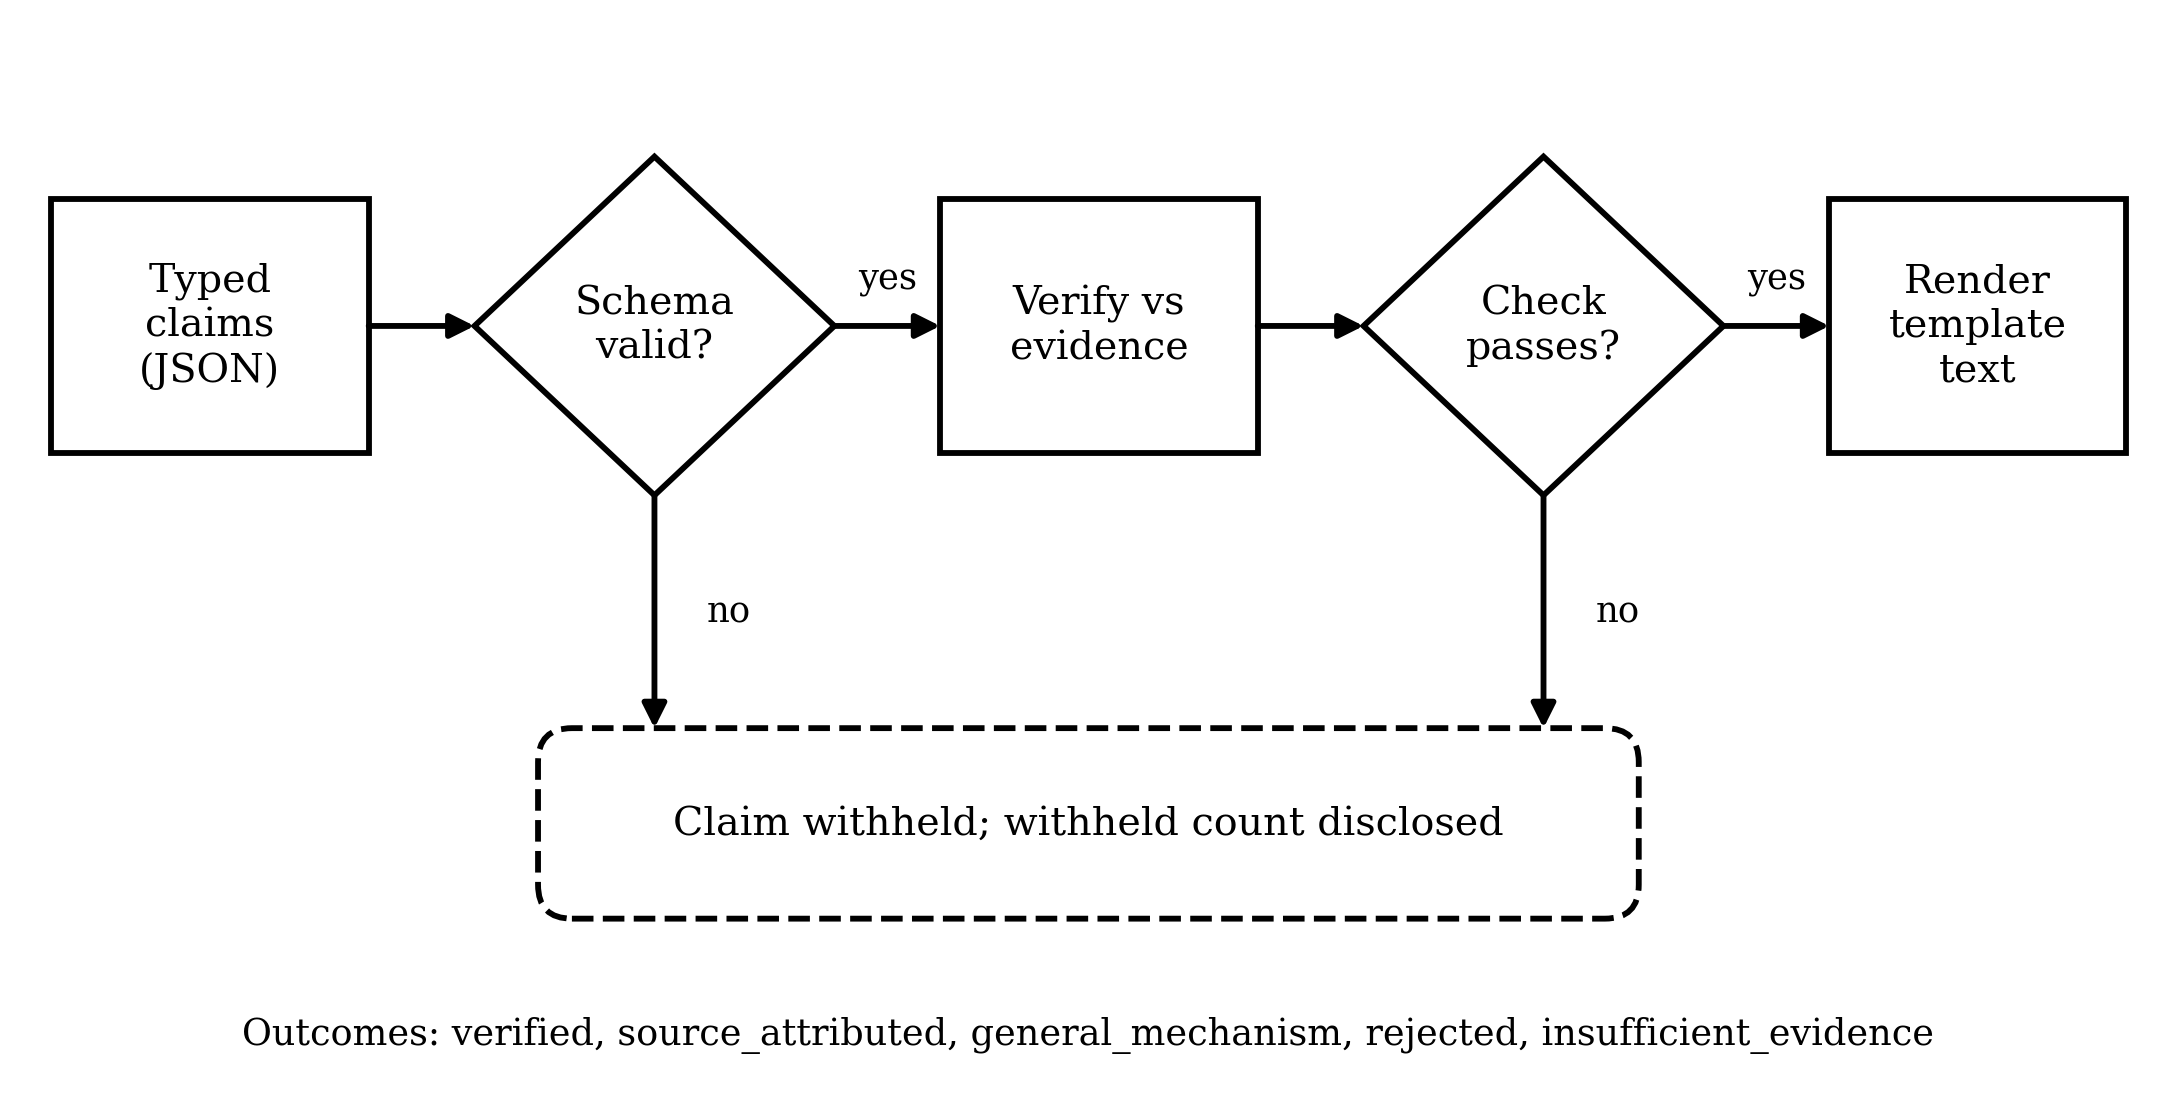
\includegraphics[width=\columnwidth]{09_claim_verification_pipeline.png}
\caption{Claim verification pipeline. The model proposes typed claims; deterministic verifiers check them against content-addressed evidence; only templated text for verified or attributed claims is rendered.}
\label{fig:verify}
\end{figure}

\paragraph{Typed claims.}
A discriminated union admits six claim types: an observation value, a rate change between two observations, the direction of a year-on-year price change, a reported explanation tied to a retrieved passage, a reviewed general mechanism, and a statistical finding tied to a registered analysis. Unknown fields are rejected, so a model cannot smuggle free text through the schema.

\paragraph{Content-addressed evidence.}
An observation identifier is the SHA-256 digest of its canonical JSON with volatile fields (retrieval time, request identifier, freshness flags) removed. A repeated retrieval of the same figure therefore keeps its identity, while a data revision or a change of definition creates a new one. Source passages are identified by the digest of their URL and text.

\paragraph{Deterministic checks.}
Numeric claims are verified in decimal arithmetic. Let $v$ be the value computed from evidence and $\hat v$ the value proposed by the model; the claim is accepted only if
\begin{equation}
\operatorname{round}_{2}(\hat v)=\operatorname{round}_{2}(v),
\label{eq:numeric}
\end{equation}
that is, the values agree at the displayed precision with no hidden floating-point tolerance. The verifier also rejects observations with conflicting values for the same period, missing dimensions or provenance, an unsupported unit, a period outside the requested scope, or a rate change between series that do not share indicator, base year, unit and source. For qualitative claims, a quotation must match a complete sentence of the source passage, which prevents deleting a preceding negation, and the rendered text states that attribution was checked but causation was not.

\paragraph{Outcomes and rendering.}
Each claim ends as \code{verified}, \code{source_attributed}, \code{general_mechanism}, \code{rejected} or \code{insufficient_evidence}. Only the first three produce text, which comes from fixed templates. The report discloses how many claims were withheld. Reports are stored in an append-only SQLite audit table with the evidence snapshot.

\paragraph{Status.}
The library is complete and unit-tested, but the current orchestrator does not call it, and its scope is limited to price statistics. Integrating it into synthesis, and extending the claim union with comparison, ranking and \emph{causal} claims bound to a graph edge and its evidence class, is the most valuable next step (\cref{sec:conclusion}). Until then, orchestrator reports are sourced but not claim-verified, and we describe them that way.

% ================================================================ VIII. eval
\section{Implementation and Evaluation}
\label{sec:eval}

\subsection{Implementation}
The backend is written in Python 3.12 with FastAPI, LangGraph for orchestration, FastMCP for tool servers, DuckDB \cite{raasveldt2019duckdb} and SQLite for storage, NetworkX \cite{hagberg2008networkx} for the graph and statsmodels \cite{seabold2010statsmodels} for Granger tests. The default models are \code{openai/gpt-oss-20b} (fast) and \code{openai/gpt-oss-120b} (reasoning), served through Groq, with an optional OpenAI path and the deterministic offline fallback. The frontend uses React 18, strict TypeScript, Vite, Tailwind and Mermaid. At the snapshot of 12 October 2026 the repository contains about 45.8k lines of Python and 11.3k lines of TypeScript. Code and data layout are described in the repository documentation\footnote{\url{https://github.com/Hariprasaadh/macrograph-ai}}.

The interface offers a chat workspace that streams one step per A2A request (\cref{fig:screen1}), a dashboard with cross-sector telemetry and citations, a causal lab with path, shockwave, twin, radar and committee tabs (\cref{fig:screen2}), and an A2A registry view.

\begin{figure*}[t]
\centering
% IMAGE 14 -- Screenshot of the chat workspace (REPLACE the placeholder file)
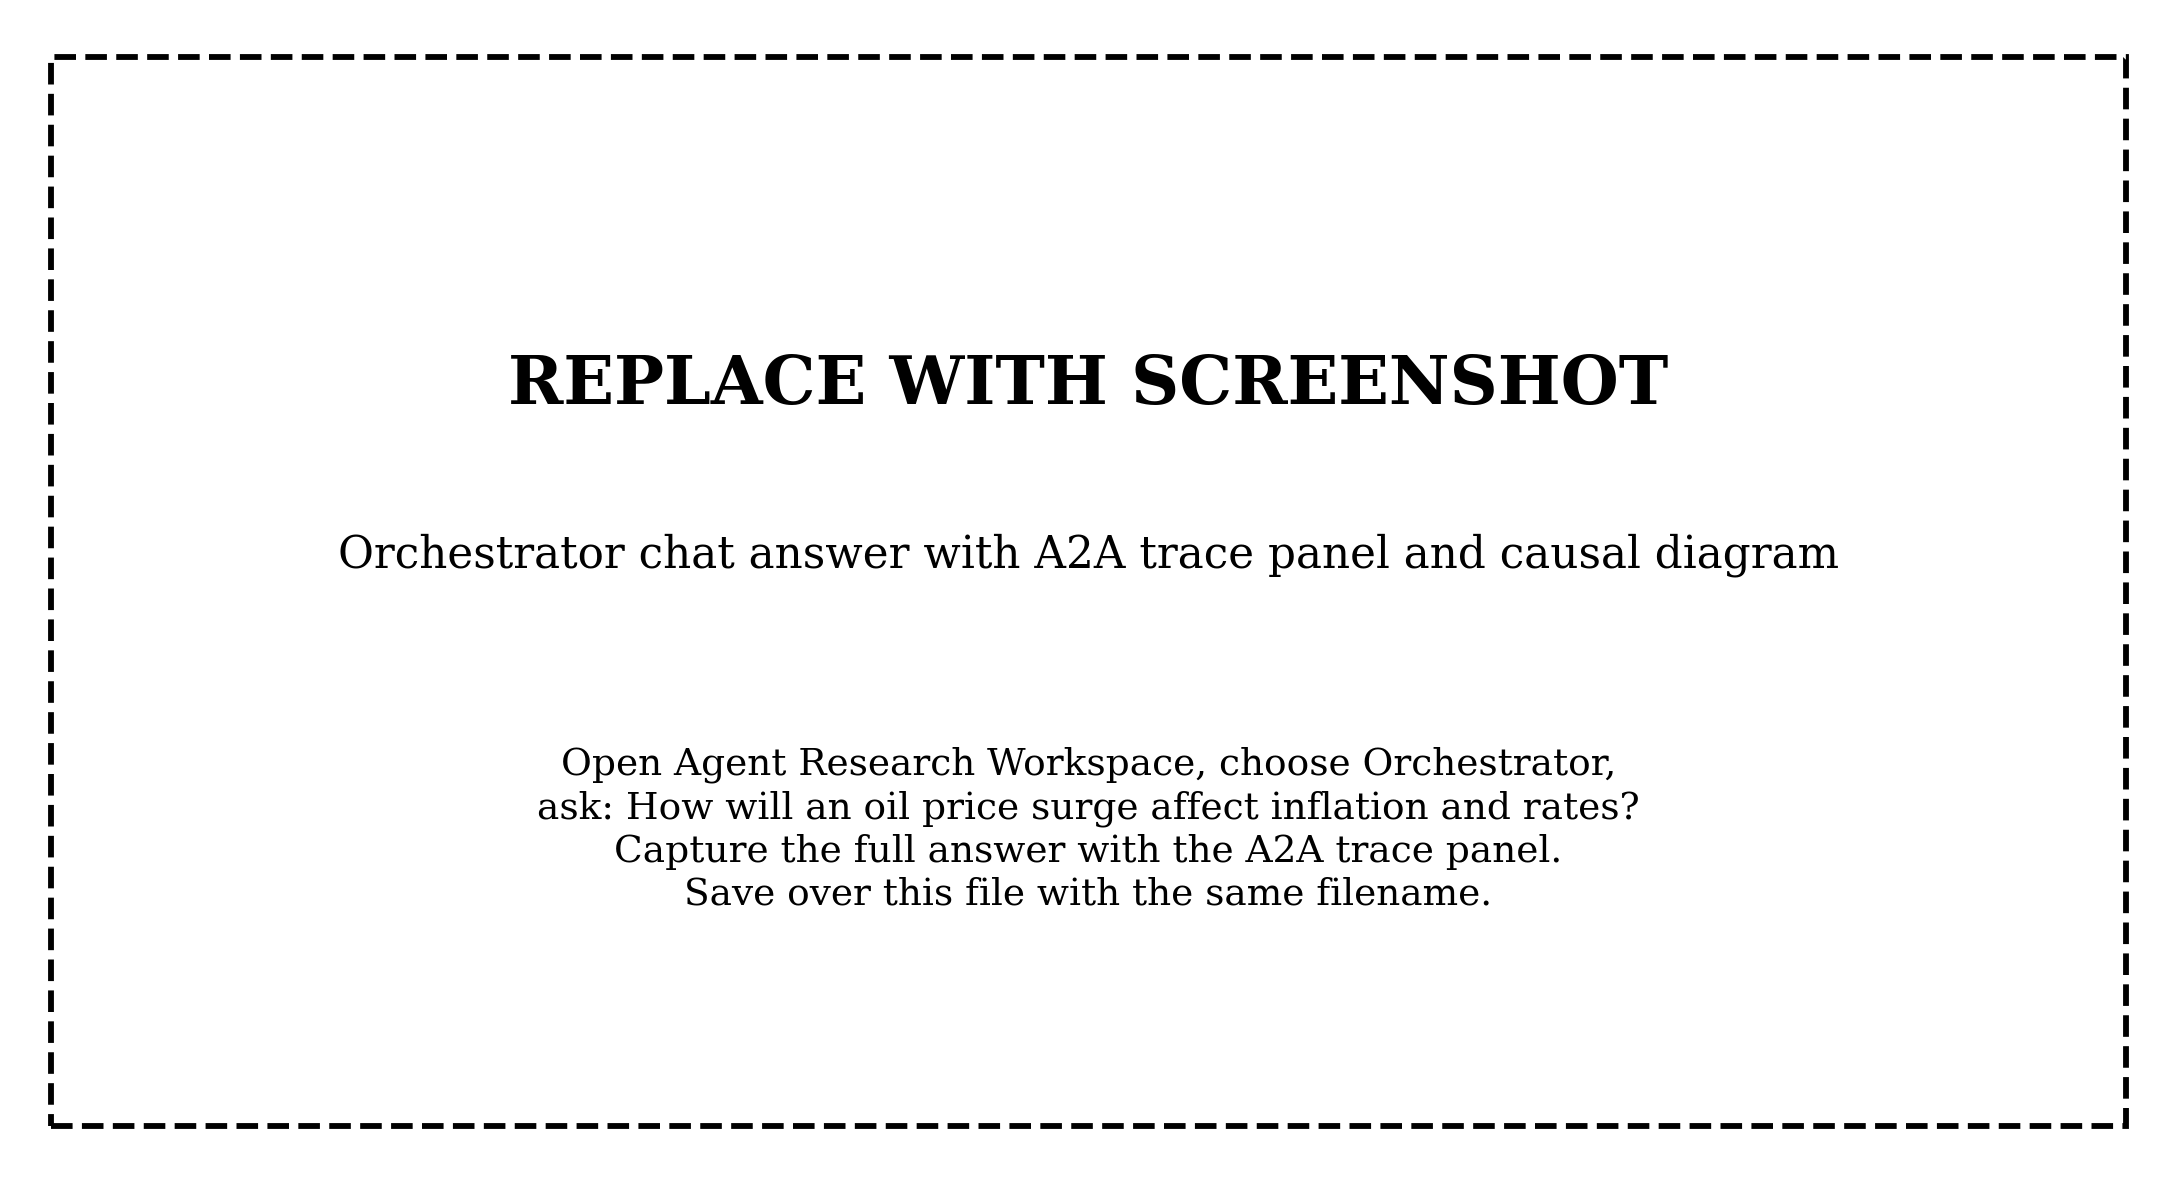
\includegraphics[width=0.72\textwidth]{14_screenshot_chat_workspace.png}
\caption{Orchestrator chat workspace showing a cited answer, the A2A trace panel and the Mermaid causal diagram for an oil-price query.}
\label{fig:screen1}
\end{figure*}

\begin{figure*}[t]
\centering
% IMAGE 15 -- Screenshot of the Causal Lab twin tab (REPLACE the placeholder file)
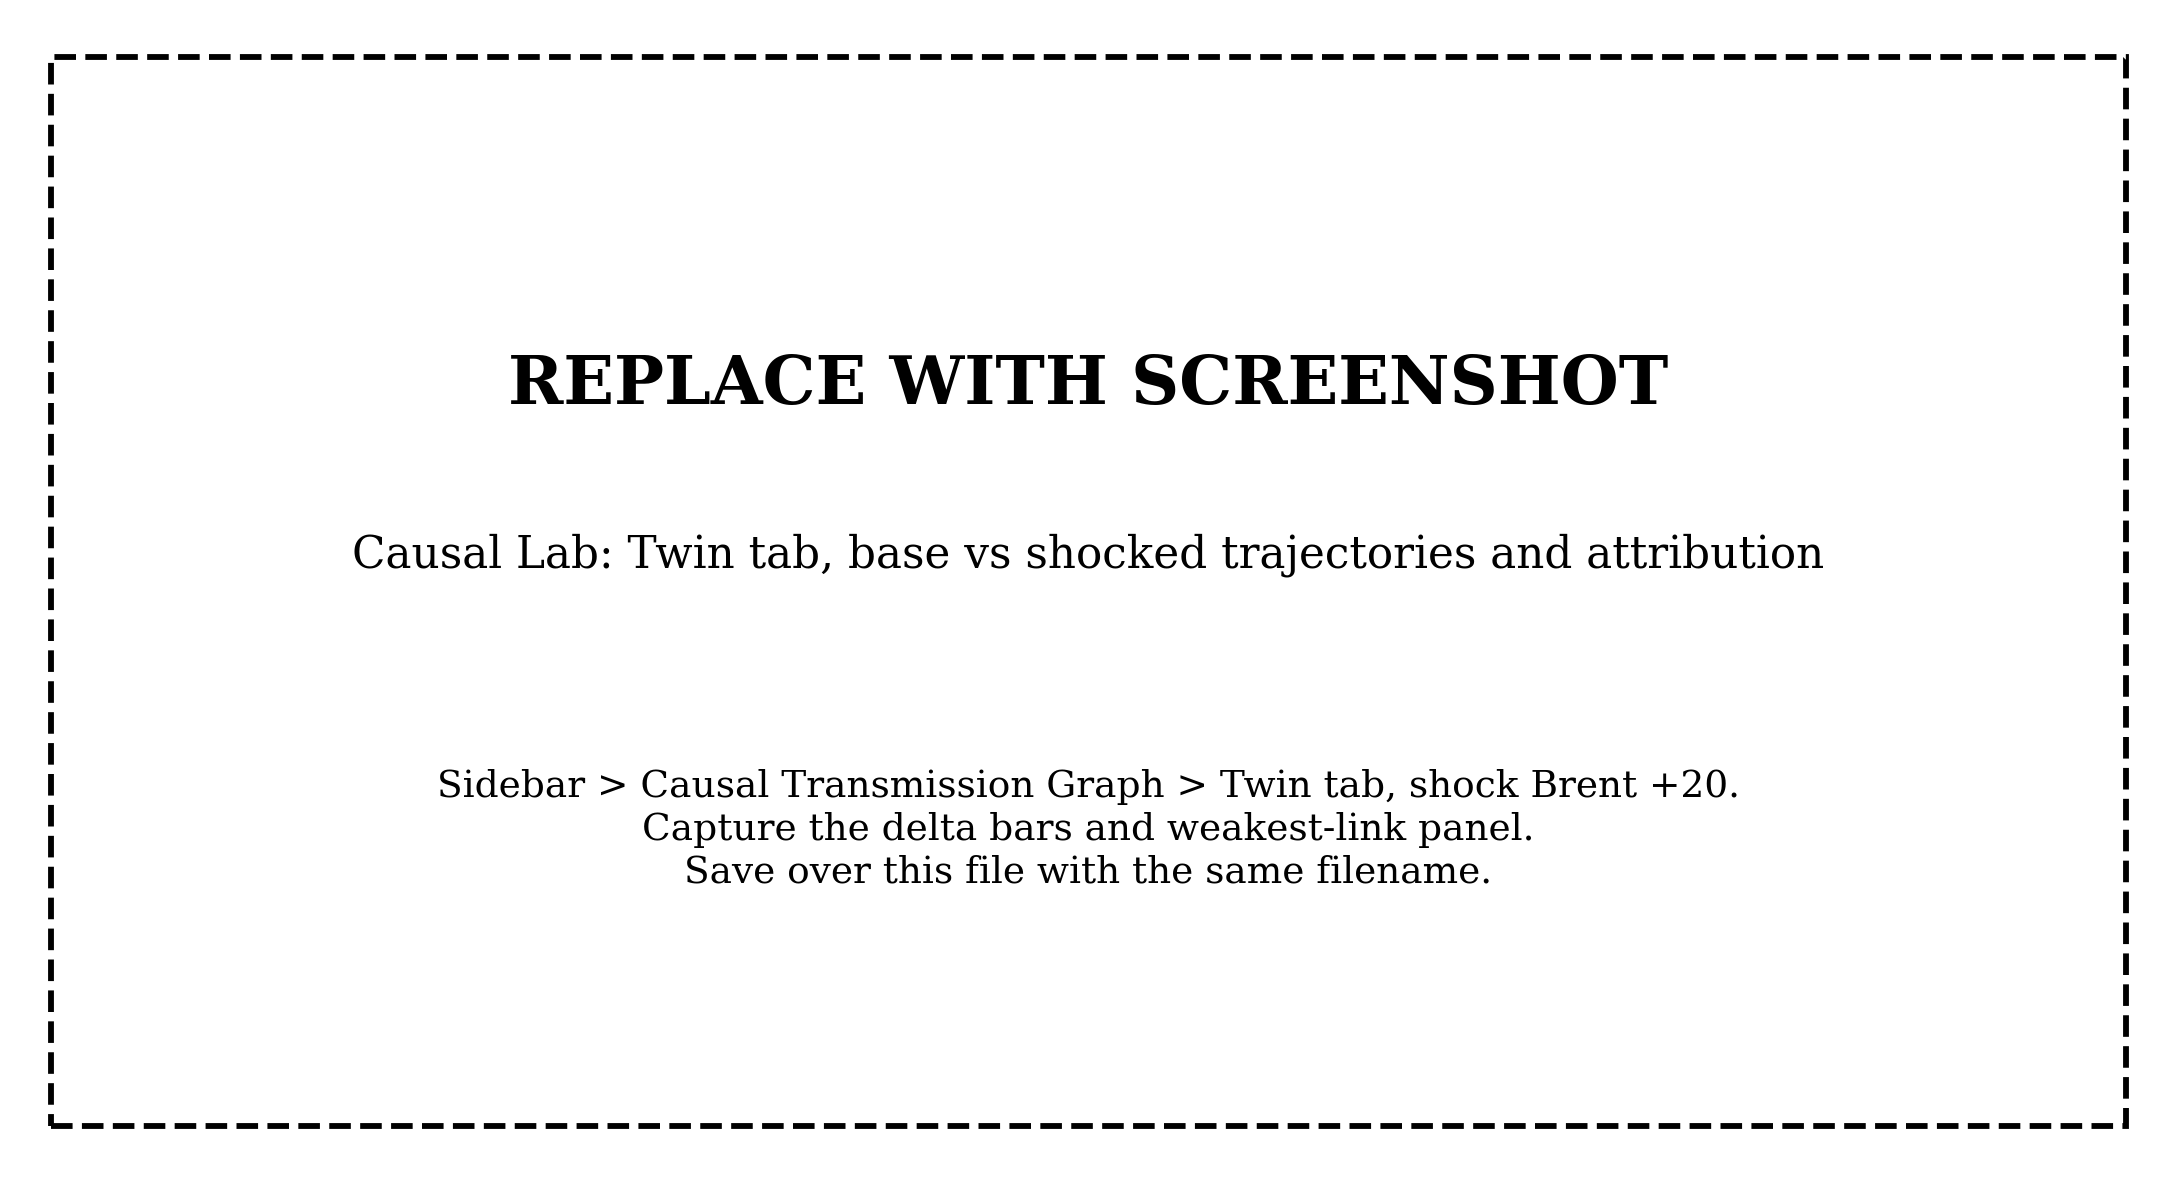
\includegraphics[width=0.72\textwidth]{15_screenshot_causal_lab.png}
\caption{Causal lab, twin tab: base and shocked trajectories, delta bars and the per-hop attribution with the weakest link highlighted.}
\label{fig:screen2}
\end{figure*}

\subsection{What has been measured}
We ran the full test suite across the ten sector packages and the core on 12 October 2026. The 455 test functions (\cref{fig:tests}) executed as 551 cases; 550 passed and one failed in 715 seconds. The failing case is in the monetary sector: a test stub for the stance fallback expects a repo rate of 5.0 while the agent returns 5.25, which indicates drift between the test and the agent's source precedence. We have not yet resolved it and report it as a known defect. Tests include regression tests for earlier bugs and pin the scenario formula, for example that the WPI delta equals $\operatorname{round}(20\cdot0.55\cdot0.95\cdot0.15,2)$. In addition, the Edge Evidence Audit and the Brent scenario above were produced by running the released code.

\begin{figure}[t]
\centering
% IMAGE 11 -- Test composition
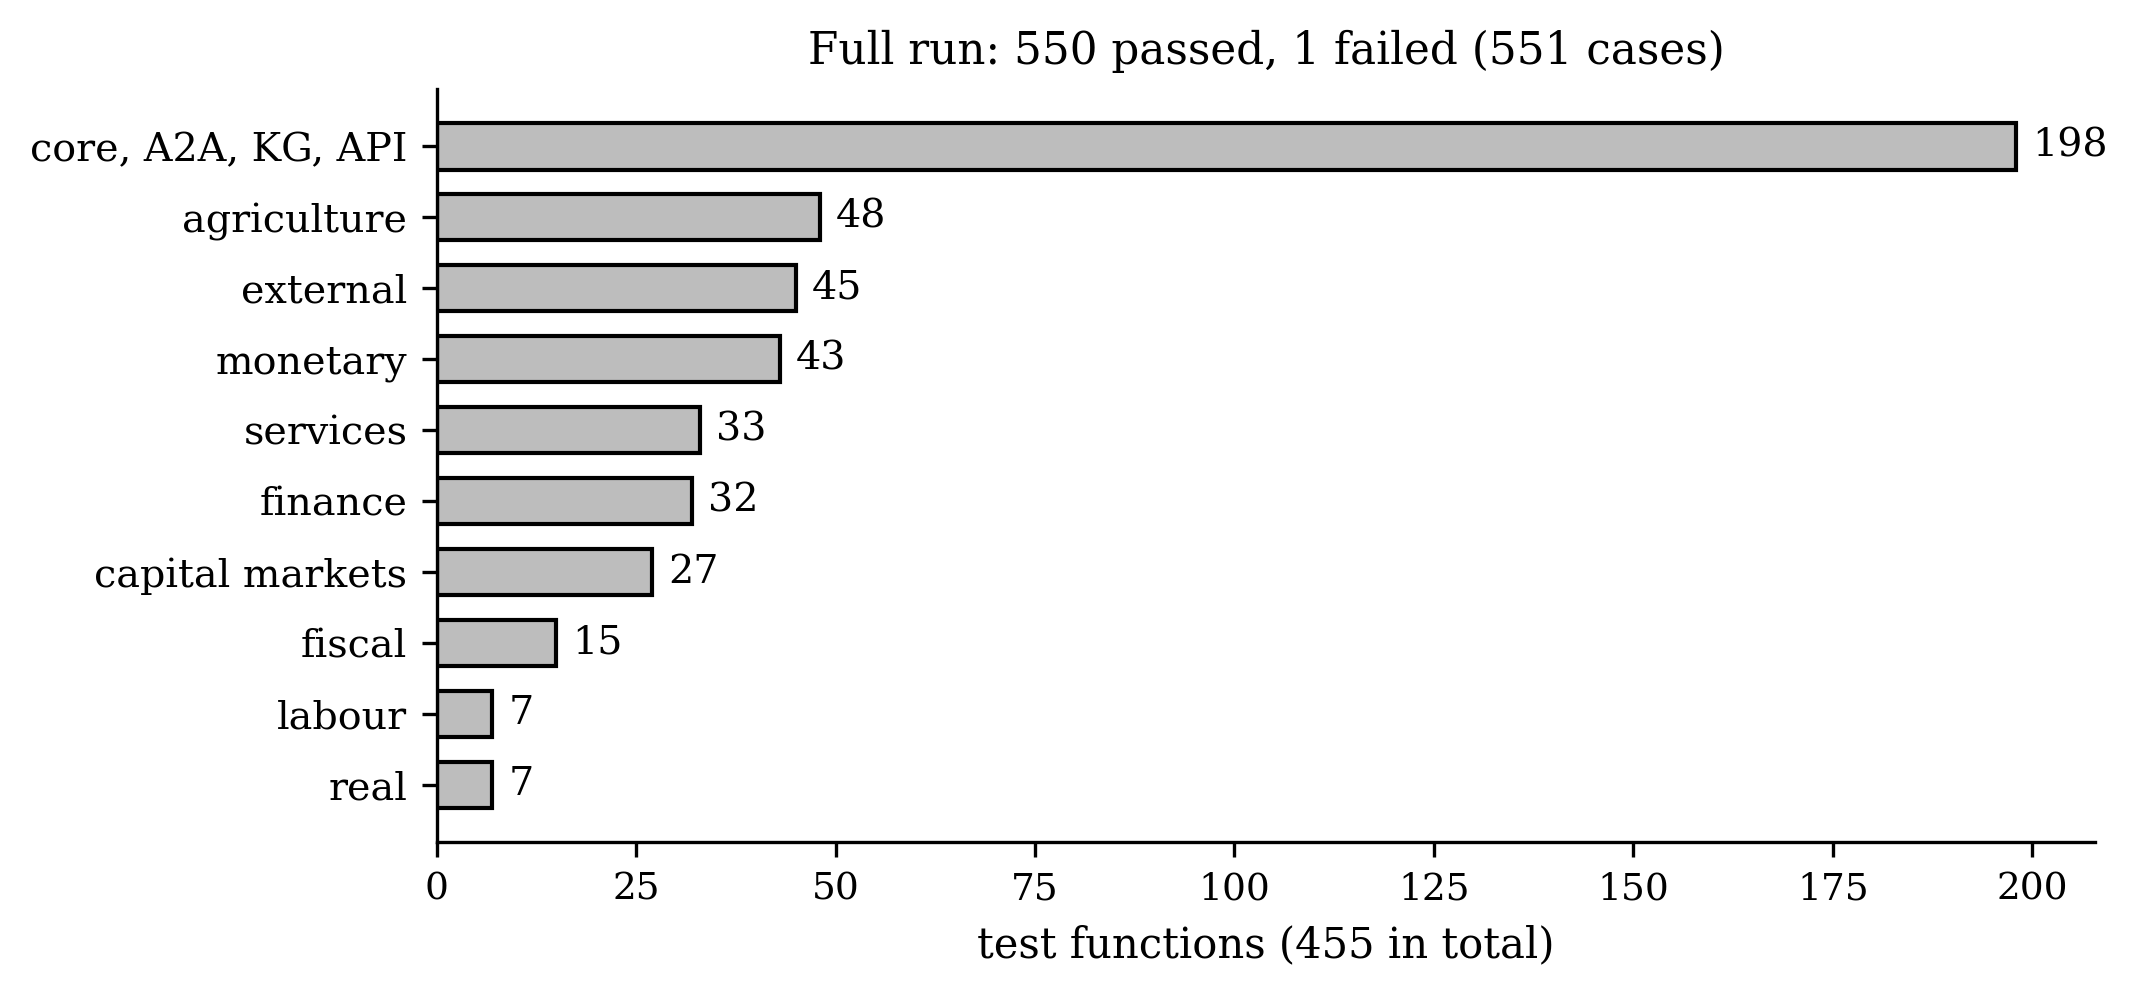
\includegraphics[width=\columnwidth]{11_test_composition.png}
\caption{Test functions by area. Sector test directories outside the default test paths were run explicitly for the full-suite result.}
\label{fig:tests}
\end{figure}

These figures show that the software behaves as specified. They are \emph{engineering} results, not evidence of answer quality. We have not yet measured whether \sys{} produces fewer unsupported statements than a baseline, whether routing selects the right agents, whether the verification gate costs coverage, or whether the committee simulator agrees with actual Monetary Policy Committee decisions. We therefore make no accuracy claim.

\subsection{Planned evaluation}
We specify the evaluation in advance so that its design cannot be tuned to the result. \Cref{fig:evalplan} summarises it.

\begin{figure}[t]
\centering
% IMAGE 13 -- Planned evaluation design
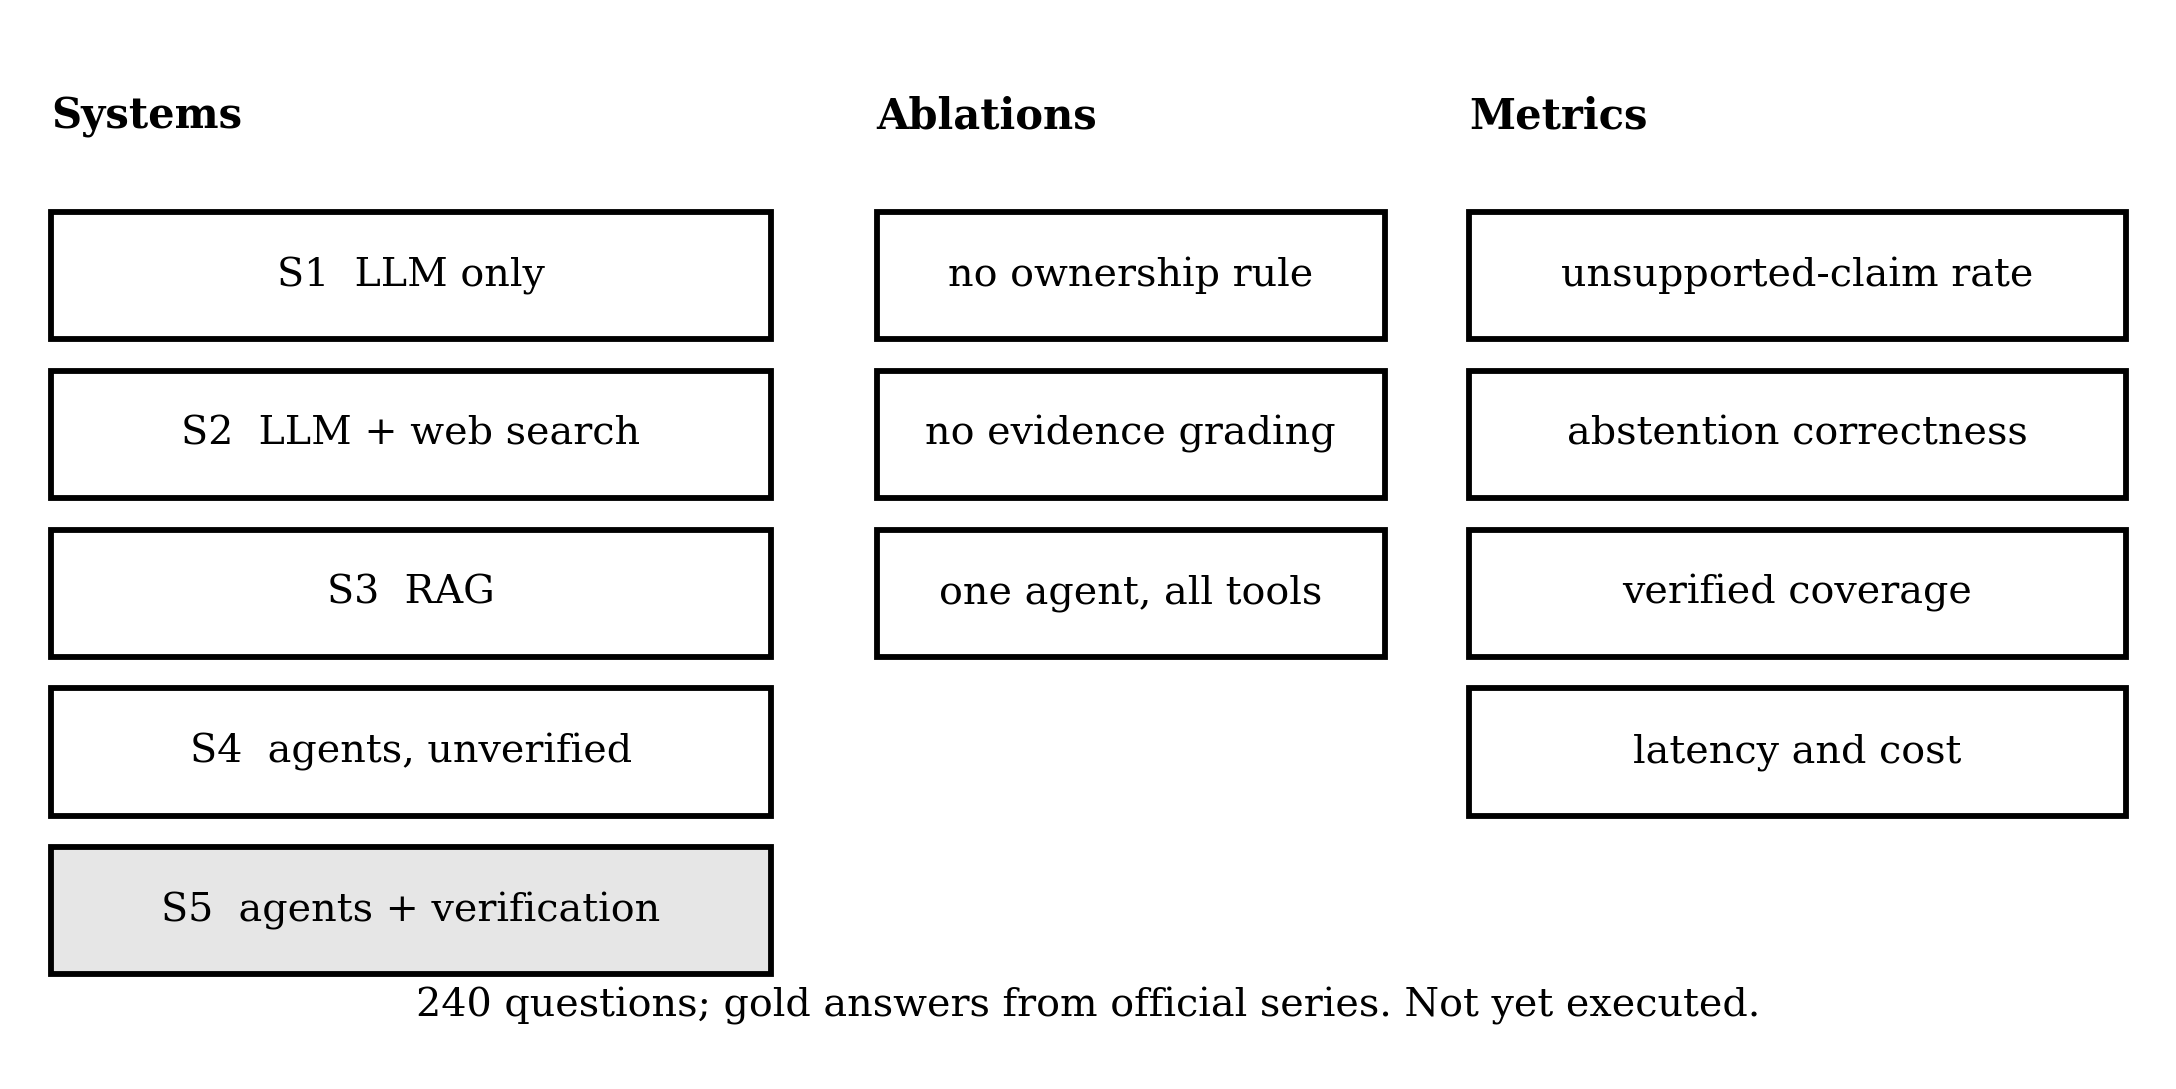
\includegraphics[width=\columnwidth]{13_planned_evaluation_design.png}
\caption{Planned evaluation (not yet executed): five systems, three ablations and four metrics over a 240-question set.}
\label{fig:evalplan}
\end{figure}

\textbf{Question set.} Table~\ref{tab:questions} lists five question types with gold answers computed directly from official series, not from model output. Unanswerable questions (data absent or a future period) test abstention.

\begin{table}[t]
\centering
\caption{Planned question set.}
\label{tab:questions}
\footnotesize
\begin{tabular}{@{}lrp{3.1cm}@{}}
\toprule
\textbf{Type} & \textbf{N} & \textbf{Gold answer from} \\
\midrule
Point lookup & 60 & Official series \\
Change / direction & 50 & Recomputed from series \\
Cross-sector synthesis & 50 & Rubric over cited indicators \\
Causal / scenario & 40 & Edge evidence class, back-test \\
Unanswerable & 40 & None (abstention) \\
\midrule
\textbf{Total} & \textbf{240} & \\
\bottomrule
\end{tabular}
\end{table}

\textbf{Systems.} S1 single LLM without tools; S2 single LLM with web search; S3 retrieval-augmented generation over the same documents; S4 multi-agent without verification (the current production path); S5 multi-agent with the verification gate. Ablations remove the ownership constraint, remove evidence grading, and replace the agents with one agent holding all tools.

\textbf{Metrics.} The primary metrics are the \emph{unsupported numeric-claim rate} (share of numeric claims in an answer that no cited observation supports), \emph{abstention correctness} on unanswerable questions, and \emph{verified-claim coverage} (the cost side of verification). Secondary metrics are citation validity, duplicate fetches and contradictory values for the same indicator within one answer, tool calls, latency and cost. We will report means with 95\% bootstrap intervals over at least three seeds and at least two LLM backends, and freeze data vintages by recording the hash of the DuckDB file with every run.

\textbf{Committee benchmark.} For the simulated committee, the ground truth is the set of decisions, vote splits and dissents published in Monetary Policy Committee resolutions since 2016. Inputs will be restricted to point-in-time data available before each meeting, and the arms will be an always-hold majority class, a Taylor-rule baseline \cite{taylor1993}, the current rule baseline, a single LLM and the three-persona LLM.

\textbf{Edge-audit evaluation.} We will extend the audit with long monthly histories, difference series to stationarity, apply Benjamini--Hochberg control across the 12 tests \cite{bh1995}, require a larger minimum sample, and report the fraction of expert-seeded edges whose estimated sign and significance survive.

% ================================================================ IX. discussion
\section{Discussion and Limitations}
\label{sec:discussion}

We list the limitations that a careful reviewer would raise, together with their status. Most come from a review of our own code.

\paragraph{Seeded statistics look like measurements.}
Edge $p$-values and confidence scores in the ontology are typed constants, and the schema's rule that a $p$-value may be absent only for \textsc{Theory} edges pushes authors to type a number for every other edge. These values feed trust scores and scenario deltas. The audit mitigates the presentation problem, because every unsupported edge is labelled, but it does not replace the constants with estimates. The correct fix is to make estimated statistics the only source and to store the sample size, estimator, window and data vintage with each edge.

\paragraph{The scenario engine is not an identified model.}
Constants are not estimated, scaling is unit-blind, the band is not an interval, and the baselines fall back to fixed defaults when no live observation exists. The right replacement is a local-projection or Bayesian VAR estimator on standardised or log-difference series with bootstrap intervals, back-tested on named episodes (the 2022 oil and Ukraine shock, the 2022--23 repo cycle, the 2013 taper episode, demonetisation in 2016 and the 2020 pandemic) against no-change and autoregressive baselines. The attenuation model would then serve as an explicit weak baseline.

\paragraph{Granger audit weaknesses.}
The audit uses a minimum overlap of only 10 months, no stationarity test, no multiple-testing correction, and takes the minimum $p$-value over lags without adjustment, which inflates false positives. Bivariate predictive causality is also not causal identification \cite{pearl2009}. The ``Granger predictive'' and ``structural'' tier names should therefore be read as aspirations until tests support them.

\paragraph{Known sign defect.}
The trade-balance to USD/INR edge has an inconsistent sign. It is annotated in the interface and in the audit, but annotation is not a fix. The ontology must be corrected and a test added that rejects any \code{EMPIRICAL} edge whose estimated sign contradicts its seeded sign.

\paragraph{Verification is not integrated.}
The library is not called by the orchestrator, and its claim types currently cover price statistics. Until it is wired into synthesis, the headline property of ``every statement is verified'' does not hold for the system, and we do not claim it.

\paragraph{Heuristic scores.}
The consensus and trust scores are ad-hoc products of fractions. They are labelled, but should be calibrated against verification outcomes (for example with a reliability diagram) or dropped.

\paragraph{Simulated committee.}
The committee is a model of archetypes, not a forecast of what the Monetary Policy Committee will do. It must not be presented as one.

\paragraph{Scope and engineering.}
The system covers one country, one family of LLM backends in the default configuration and a graph of 20 nodes. Several modules exceed the project's 400-line guideline, some silent failure paths still exist in optional components, the cost-bearing endpoints have no authentication or rate limit, and the A2A trace is in memory only. Documentary evidence (RAG over policy documents and minutes) is not implemented, so qualitative explanations rest on sector reports and search excerpts. These are tracked in the repository's status document.

\paragraph{Ethics and use.}
\sys{} is a research system for analysts and not investment advice. Outputs depend on third-party data terms; releasing frozen data snapshots requires checking each source's licence. LLM providers receive the query text and the evidence the agent sends, so deployments handling sensitive queries should use a provider and a configuration that meet their data-handling requirements.

% ================================================================ X. conclusion
\section{Conclusion and Future Work}
\label{sec:conclusion}

We described \sys{}, a multi-agent platform for Indian macroeconomic analysis whose reliability comes from structure: one owner per indicator, a closed set of declared agent-to-agent edges, a protocol that refuses sourceless responses, an evidence-graded causal graph and a verification library that renders only checked text. Our own audit shows where the structure is still ahead of the evidence: none of the 12 causal edges can be tested on the bundled data, the scenario engine is a heuristic baseline, and claim verification is not yet part of the production path. We regard that candour as part of the contribution, because it turns implicit weaknesses into measurable ones.

\Cref{fig:gate} shows the next architectural step: the model proposes typed claims, a verification gate checks them, and a causal claim is bound to a graph edge and its evidence class, so that a \code{SEEDED} edge is hedged and an \code{EMPIRICAL} one is cited with its sample size. The work plan has four parts: (i) wire verification into synthesis and extend the claim union; (ii) estimate edges from long monthly series with stationarity handling and multiple-testing control; (iii) replace the attenuation heuristic by a local-projection estimator and back-test it; (iv) run the evaluation of \cref{sec:eval} with point-in-time data. A public Indian macroeconomic verification benchmark would be a useful artifact for the community regardless of how \sys{} performs on it.

\begin{figure}[t]
\centering
% IMAGE 12 -- Proposed verification gate (future work)
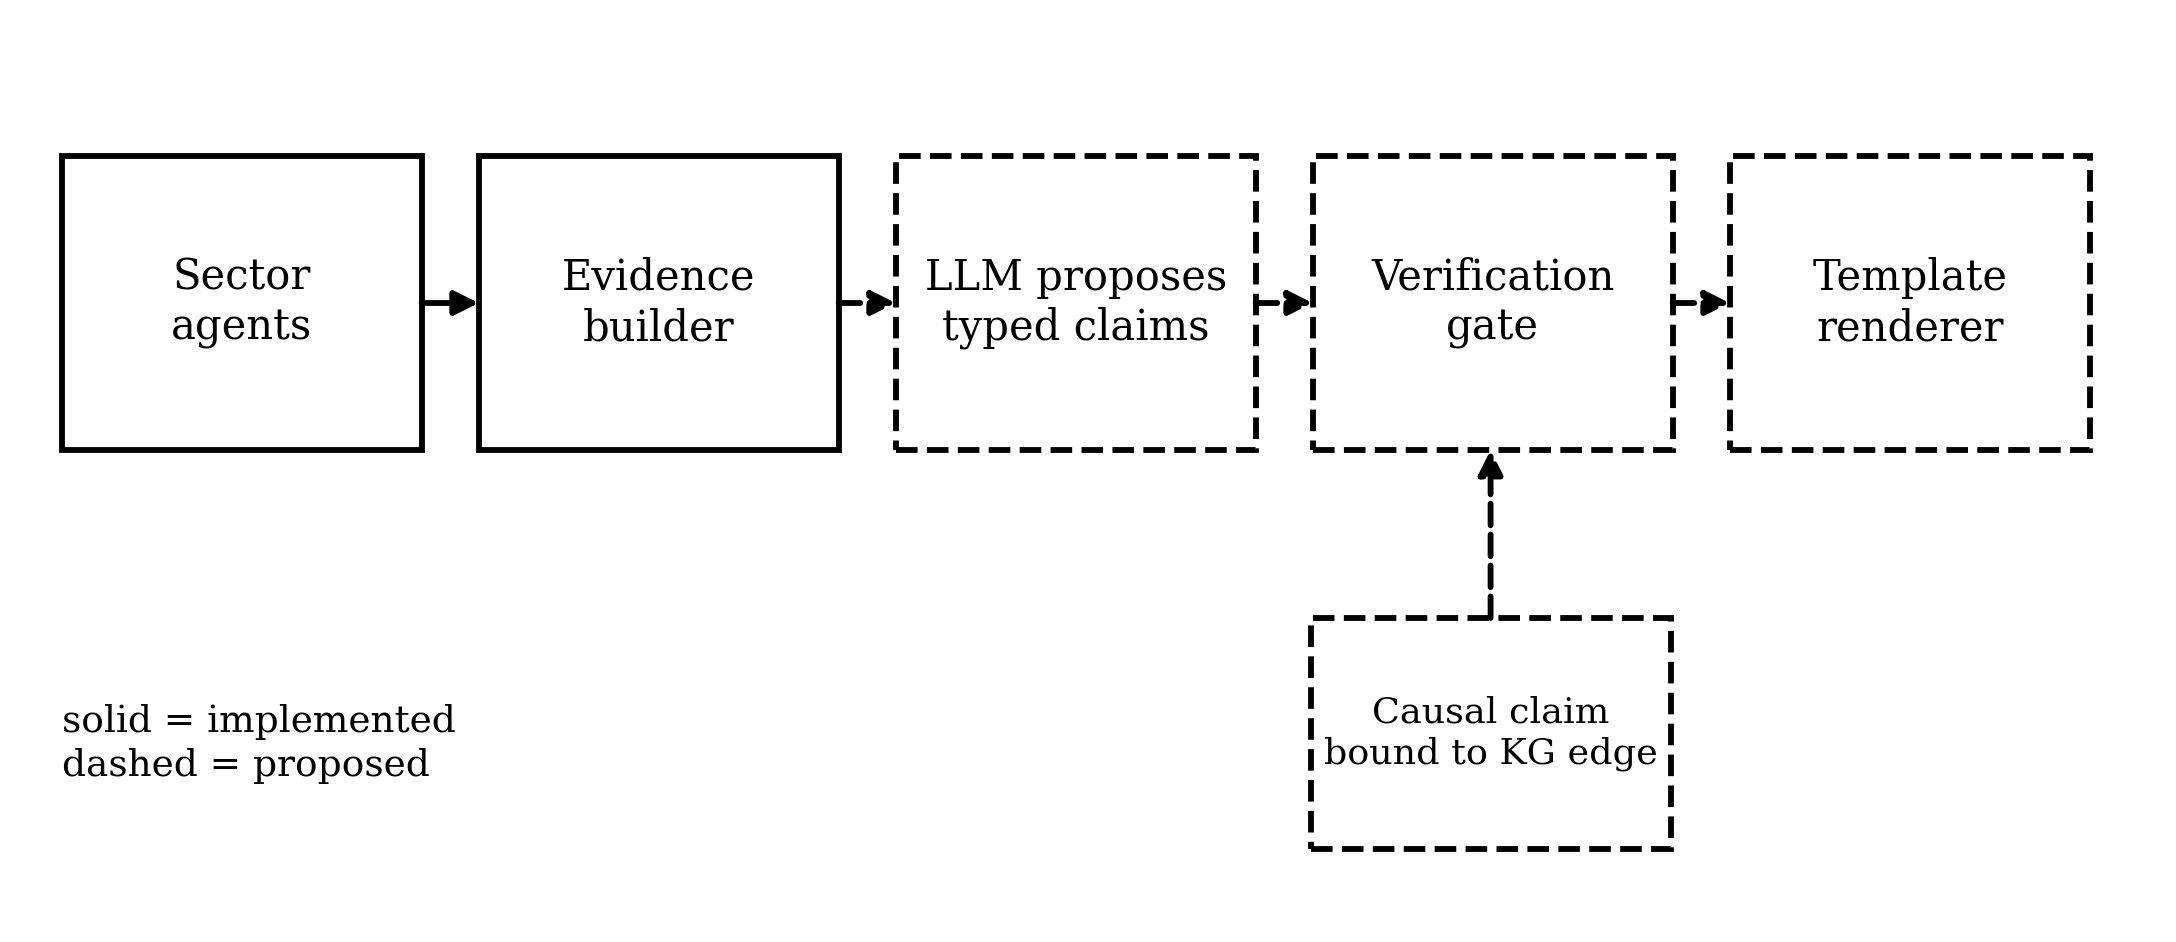
\includegraphics[width=\columnwidth]{12_proposed_verification_gate.png}
\caption{Proposed architecture with a verification gate (dashed boxes are future work). Causal claims are bound to a graph edge and its evidence class.}
\label{fig:gate}
\end{figure}

\section*{Reproducibility}
The code, documentation and test suite are in the project repository. Offline operation without API keys is supported, so the architecture, protocol, graph, scenario and audit results in this paper can be reproduced without paid services. Live-data results depend on the state of public statistical sources on the date of the run, so we record the data snapshot with each evaluation run.

\section*{Declaration on AI Assistance}
Parts of the software, the figures and the first draft of this manuscript were prepared with an AI coding assistant (Claude, Anthropic). The authors reviewed and edited the text, verified the reported measurements by running the released code, and take responsibility for all content, including the references, which must be checked against the original sources. \todo{Adapt this statement to the target venue's AI-use policy.}

\section*{Acknowledgment}
The authors thank their project guide, Dr.\ Tulasi Prasad Sariki, for guidance throughout this work, which was carried out for the course BCSE497J (Project~I) at Vellore Institute of Technology, Chennai. \todo{Add funding information, if any.}

% ================================================================ references
\begin{thebibliography}{99}
\bibitem{ji2023hallucination} Z.~Ji \emph{et al.}, ``Survey of hallucination in natural language generation,'' \emph{ACM Comput. Surv.}, vol.~55, no.~12, art.~248, 2023.
\bibitem{rashkin2023ais} H.~Rashkin \emph{et al.}, ``Measuring attribution in natural language generation models,'' \emph{Comput. Linguist.}, vol.~49, no.~4, pp.~777--840, 2023.
\bibitem{gao2023alce} T.~Gao, H.~Yen, J.~Yu, and D.~Chen, ``Enabling large language models to generate text with citations,'' in \emph{Proc. EMNLP}, 2023.
\bibitem{li2024econagent} N.~Li \emph{et al.}, ``EconAgent: Large language model-empowered agents for simulating macroeconomic activities,'' in \emph{Proc. 62nd Annu. Meeting Assoc. Comput. Linguist. (ACL)}, 2024.
\bibitem{xiao2024tradingagents} Y.~Xiao, E.~Sun, D.~Luo, and W.~Wang, ``TradingAgents: Multi-agents LLM financial trading framework,'' arXiv:2412.20138, 2025.
\bibitem{hao2025mlab} Y.~Hao and D.~Xie, ``A multi-LLM-agent-based framework for economic and public policy analysis,'' arXiv:2502.16879, 2025.
\bibitem{kato2026aieconomist} M.~Kato, ``AI Economist Agent: An agentic framework for model-grounded economic analysis with RAG, knowledge graphs, and large language models,'' arXiv:2606.20041, 2026.
\bibitem{lin2026expectations} J.~Lin, L.~Sun, and Y.~Yan, ``Simulating macroeconomic expectations in survey experiments with LLM-based economic agents,'' arXiv:2505.17648, 2026.
\bibitem{zheng2022aieconomist} S.~Zheng \emph{et al.}, ``The AI Economist: Taxation policy design via two-level deep multiagent reinforcement learning,'' \emph{Sci. Adv.}, vol.~8, no.~18, eabk2607, 2022.
\bibitem{wu2023bloomberggpt} S.~Wu \emph{et al.}, ``BloombergGPT: A large language model for finance,'' arXiv:2303.17564, 2023.
\bibitem{yao2023react} S.~Yao \emph{et al.}, ``ReAct: Synergizing reasoning and acting in language models,'' in \emph{Proc. ICLR}, 2023.
\bibitem{park2023generative} J.~S. Park \emph{et al.}, ``Generative agents: Interactive simulacra of human behavior,'' in \emph{Proc. ACM UIST}, 2023.
\bibitem{wu2023autogen} Q.~Wu \emph{et al.}, ``AutoGen: Enabling next-gen LLM applications via multi-agent conversation,'' arXiv:2308.08155, 2023.
\bibitem{hong2024metagpt} S.~Hong \emph{et al.}, ``MetaGPT: Meta programming for a multi-agent collaborative framework,'' in \emph{Proc. ICLR}, 2024.
\bibitem{wang2024agentsurvey} L.~Wang \emph{et al.}, ``A survey on large language model based autonomous agents,'' \emph{Front. Comput. Sci.}, vol.~18, no.~6, art.~186345, 2024.
\bibitem{guo2024masurvey} T.~Guo \emph{et al.}, ``Large language model based multi-agents: A survey of progress and challenges,'' in \emph{Proc. IJCAI (Survey Track)}, 2024.
\bibitem{mcp2024} Anthropic, ``Model Context Protocol specification,'' 2024. [Online]. Available: \url{https://modelcontextprotocol.io}
\bibitem{a2a2025} Google, ``Announcing the Agent2Agent (A2A) protocol,'' Google Developers Blog, 2025. [Online]. Available: \url{https://developers.googleblog.com}
\bibitem{lewis2020rag} P.~Lewis \emph{et al.}, ``Retrieval-augmented generation for knowledge-intensive NLP tasks,'' in \emph{Proc. NeurIPS}, vol.~33, 2020, pp.~9459--9474.
\bibitem{edge2024graphrag} D.~Edge \emph{et al.}, ``From local to global: A graph RAG approach to query-focused summarization,'' arXiv:2404.16130, 2024.
\bibitem{zhu2025kg2rag} X.~Zhu, Y.~Xie, Y.~Liu, Y.~Li, and W.~Hu, ``Knowledge graph-guided retrieval augmented generation,'' arXiv:2502.06864, 2025.
\bibitem{pan2024llmkg} S.~Pan \emph{et al.}, ``Unifying large language models and knowledge graphs: A roadmap,'' \emph{IEEE Trans. Knowl. Data Eng.}, vol.~36, no.~7, pp.~3580--3599, 2024.
\bibitem{dadopoulos2025metadata} M.~Dadopoulos, A.~Ladas, I.~Negkakis, and S.~Moschidis, ``Metadata-driven retrieval-augmented generation for financial question answering,'' arXiv:2510.24402, 2025.
\bibitem{yang2020kgmacro} Y.~Yang, Y.~Pang, G.~Huang, and W.~E, ``The knowledge graph for macroeconomic analysis with alternative big data,'' SSRN Working Paper 3707964, 2020.
\bibitem{thorne2018fever} J.~Thorne, A.~Vlachos, C.~Christodoulopoulos, and A.~Mittal, ``FEVER: A large-scale dataset for fact extraction and VERification,'' in \emph{Proc. NAACL-HLT}, 2018.
\bibitem{belhajjame2013prov} K.~Belhajjame \emph{et al.}, ``PROV-DM: The PROV data model,'' W3C Recommendation, Apr. 2013.
\bibitem{granger1969} C.~W.~J. Granger, ``Investigating causal relations by econometric models and cross-spectral methods,'' \emph{Econometrica}, vol.~37, no.~3, pp.~424--438, 1969.
\bibitem{sims1980macro} C.~A. Sims, ``Macroeconomics and reality,'' \emph{Econometrica}, vol.~48, no.~1, pp.~1--48, 1980.
\bibitem{jorda2005lp} \`O.~Jord\`a, ``Estimation and inference of impulse responses by local projections,'' \emph{Amer. Econ. Rev.}, vol.~95, no.~1, pp.~161--182, 2005.
\bibitem{dickey1979} D.~A. Dickey and W.~A. Fuller, ``Distribution of the estimators for autoregressive time series with a unit root,'' \emph{J. Amer. Statist. Assoc.}, vol.~74, no.~366, pp.~427--431, 1979.
\bibitem{kpss1992} D.~Kwiatkowski, P.~C.~B. Phillips, P.~Schmidt, and Y.~Shin, ``Testing the null hypothesis of stationarity against the alternative of a unit root,'' \emph{J. Econometrics}, vol.~54, pp.~159--178, 1992.
\bibitem{bh1995} Y.~Benjamini and Y.~Hochberg, ``Controlling the false discovery rate: A practical and powerful approach to multiple testing,'' \emph{J. R. Statist. Soc. B}, vol.~57, no.~1, pp.~289--300, 1995.
\bibitem{pearl2009} J.~Pearl, \emph{Causality: Models, Reasoning, and Inference}, 2nd~ed. Cambridge, U.K.: Cambridge Univ. Press, 2009.
\bibitem{taylor1993} J.~B. Taylor, ``Discretion versus policy rules in practice,'' \emph{Carnegie-Rochester Conf. Ser. Public Policy}, vol.~39, pp.~195--214, 1993.
\bibitem{raasveldt2019duckdb} M.~Raasveldt and H.~M\"uhleisen, ``DuckDB: An embeddable analytical database,'' in \emph{Proc. ACM SIGMOD}, 2019, pp.~1981--1984.
\bibitem{hagberg2008networkx} A.~A. Hagberg, D.~A. Schult, and P.~J. Swart, ``Exploring network structure, dynamics, and function using NetworkX,'' in \emph{Proc. 7th Python in Science Conf. (SciPy)}, 2008, pp.~11--15.
\bibitem{seabold2010statsmodels} S.~Seabold and J.~Perktold, ``statsmodels: Econometric and statistical modeling with Python,'' in \emph{Proc. 9th Python in Science Conf. (SciPy)}, 2010.
\end{thebibliography}

% ================================================================ appendix
\appendices
\section{Reproducing the reported results}
\label{app:repro}
From the repository root, in a Python 3.12 environment with the project dependencies installed:
\begin{itemize}
\item the default test suite is run with \code{pytest}; the sector suites outside the default test paths are listed in the repository documentation;
\item the Brent scenario of \cref{tab:brent} is produced by calling \code{causal_engine.simulate_scenario("Brent +20", "in.macro.prices.brent_crude", 20.0)};
\item the audit of \cref{fig:audit} is produced by \code{core.research.edge_audit.audit_edges()}.
\end{itemize}

\section{Evidence-class vocabulary}
\label{app:labels}
\begin{list}{}{\setlength{\leftmargin}{0pt}\setlength{\labelwidth}{0pt}\setlength{\itemindent}{0pt}\setlength{\labelsep}{0pt}\setlength{\itemsep}{2pt}\setlength{\parsep}{0pt}\setlength{\topsep}{2pt}}
\item \code{LIVE}: value fetched at request time from a source.
\item \code{CACHED}: stored copy with its publication reference.
\item \code{SIM}: computed in memory by a simulator; never written to a sector store.
\item \code{SEEDED}: constant typed into the ontology, not estimated.
\item \code{EMPIRICAL}: edge statistic estimated by the audit from series data.
\item \code{UNTESTABLE_N} / \code{UNTESTABLE_NO_DATA}: too few overlapping observations, or none.
\item \code{heuristic}: score built from fractions with fixed weights; not calibrated.
\end{list}

\end{document}
